% =============================================================================
%  A Unified Mathematical Framework for Substrate-Agnostic Emergent Systems
%  IEEE-style LaTeX source. Compile with: pdflatex emergent_systems.tex
%  (run twice for cross-references)
% =============================================================================
\documentclass[journal]{IEEEtran}

% ---------- Encoding & fonts ----------
\usepackage[utf8]{inputenc}
\usepackage[T1]{fontenc}
% \usepackage{lmodern}  % Optional; uncomment if you have lmodern installed (most full TeX distributions do).
\usepackage[expansion=false]{microtype}  % drop "expansion=false" if you have lmodern or another scalable font

% ---------- Math ----------
\usepackage{amsmath, amssymb, amsthm, mathtools}

% ---------- Layout and references ----------
\usepackage{enumitem}
\usepackage{cite}
\usepackage{url}
\usepackage{tikz}
\usetikzlibrary{arrows.meta,positioning}

% ---------- Hyperlinks ----------
\usepackage[hidelinks]{hyperref}

% ---------- Theorem environments ----------
\theoremstyle{plain}
\newtheorem{theorem}{Theorem}[section]
\newtheorem{proposition}[theorem]{Proposition}
\newtheorem{lemma}[theorem]{Lemma}

\theoremstyle{definition}
\newtheorem{definition}[theorem]{Definition}

% Conjectures and open problems use named labels (C1, C2, ...; OP1, OP2, ...).
% We define unnumbered theorem-like environments and provide the label manually.
\theoremstyle{plain}
\newtheorem*{conjecturestar}{Conjecture}
\newtheorem*{openproblemstar}{Open Problem}

% Convenience: a conjecture/open-problem with an explicit short tag.
\newenvironment{namedconjecture}[1]{%
  \begin{conjecturestar}[#1]%
}{\end{conjecturestar}}
\newenvironment{namedopenproblem}[1]{%
  \begin{openproblemstar}[#1]%
}{\end{openproblemstar}}

% ---------- Research-note environment ----------
\newenvironment{implnote}[1][Computational implication]{%
  \par\smallskip\noindent\emph{#1.}\ }{\par\smallskip}

% Local topic headings avoid IEEEtran's visually heavy "1)" subsubsection
% style while still creating anchors for cross-references.
\newcounter{topic}[subsection]
\renewcommand{\thetopic}{\thesubsection.\arabic{topic}}
\newcommand{\topic}[1]{%
  \refstepcounter{topic}%
  \par\smallskip\noindent\textbf{#1.}\ }

% ---------- Math shortcuts ----------
\DeclareMathOperator{\EI}{EI}
\DeclareMathOperator{\CE}{CE}
\DeclareMathOperator{\KL}{KL}
\DeclareMathOperator{\Param}{Param}
\DeclareMathOperator{\supp}{supp}
\newcommand{\Hmax}{\mathbf{H}_{\max}}
\newcommand{\R}{\mathbb{R}}
\newcommand{\N}{\mathbb{N}}
\newcommand{\Pmeas}{\mathcal{P}}
\newcommand{\Mplus}{\mathcal{M}_{+}}
\newcommand{\X}{\mathbf{X}}

% =============================================================================
\title{A Mathematical Theory of Life as the Categorical Structure of Substrate-Agnostic Emergent Systems Observed by an Independent Observer}
\author{Liam~McGuire%
\thanks{Liam McGuire is an unaffiliated researcher. Address:
Seattle, Washington, United States. Email: liammcg44@gmail.com.}}

\begin{document}
\maketitle

\begin{abstract}
This paper proposes a substrate-agnostic mathematical theory of life as the
categorical structure of certain emergent stochastic systems observed by an
independent observer. A system is a 4-tuple
$\mathcal{S} = (\mathbf{X}, V, F, T)$ --- substrate, variation, viability
filter, interaction topology --- and an observer is a category-theoretic
functor $O : \mathbf{Sys} \to \mathbf{Obs}$ applied to the system's
trajectory. The ambient category $\mathbf{Sys}$ is committed to the symmetric
monoidal category of algebras over the operad of wiring diagrams, with values
in a Markov category of measurable spaces. A system--observer pair is
\emph{alive} iff it satisfies three intrinsic conditions: non-trivial macro
causal structure (Hoel-style causal emergence positive), entity persistence
across a window, and a search-hierarchy depth at level one or higher with
discriminative capacity at each level. The full vitality profile
$(k, \boldsymbol{\sigma})$ --- depth $k$ plus a level-indexed self-reference
vector $\boldsymbol{\sigma}$ --- is reported as an attribute of each member.
The framework states four central conjectures: sufficiency (some 4-tuple
system is alive), necessity (every life-producing pair decomposes as a
4-tuple system in the operadic ambient), characterisation (the two are
equivalent), and level emergence (the structural mechanism by which
hierarchies arise dynamically). Composition is two-axis: vertical via the
recursive level structure, and horizontal via the substrate-composition
operator $\boxtimes_\kappa$. The framework is intended as a theory that
\emph{predicts} life across substrates --- biological, programmatic, and
cultural alike --- not as a vocabulary that re-describes existing
artificial-life systems.
\end{abstract}

\begin{IEEEkeywords}
Artificial life, categorical biology, causal emergence, level emergence,
operad of wiring diagrams, substrate-agnostic systems, vitality profile.
\end{IEEEkeywords}

\section{Introduction}

What is life, mathematically? This paper takes the question seriously and
proposes a precise answer that does not depend on what substance the life
is made of. The answer it commits to is roughly this: life is the
categorical structure of a particular kind of mathematical object --- a
recursively built, stochastic, compositional system whose internal dynamics
admit a precise numerical classification, and which is \emph{recognised as
alive} by an external observer.

Concretely, a system is a 4-tuple $\mathcal{S} = (\mathbf{X}, V, F, T)$
consisting of a substrate $\mathbf{X}$, a variation operator $V$, a
viability filter $F$, and an interaction topology $T$, iterating on a joint
state space $Z = X \times \Mplus(X)$ via
$(x_{t+1}, \mu_{t+1}) = (\widetilde S_F \circ \widetilde V_T \circ
\widetilde\Phi)(x_t, \mu_t)$. An observer is a category-theoretic functor
$O : \mathbf{Sys} \to \mathbf{Obs}$, external to the system, that watches
the trajectory and produces an observation record. The category $\mathbf{Sys}$
is committed to the symmetric monoidal category of $\mathcal{O}_W$-algebras
in a Markov category $\mathbf{Stoch}$, where $\mathcal{O}_W$ is the operad
of wiring diagrams of Vagner, Spivak \& Lerman~\cite{vagner2015algebras}.
A system--observer pair is in the category of alive things
$\mathbf{LifeCat}$ when its trajectory exhibits non-trivial macro causal
structure (Hoel-style causal emergence positive), entity persistence, and
a search hierarchy of depth at least one. The vitality profile
$(k, \boldsymbol{\sigma})$ --- depth $k$ plus level-indexed self-reference
$\boldsymbol{\sigma}$ --- is reported as a structural attribute.

The proposed framework is \textbf{predictive, not descriptive}. It treats
life as a substrate-agnostic structural fact about a system, and biological
life as one specific realisation. The framework predicts that the same
categorical structure underlies programmatic life (e.g.\ self-replicating
programs subject to mutation and selection, as in Tierra), hybrid
biological--computational life (e.g.\ cells coupled to foundation-model
observers), cultural and linguistic life (the structural depth of which
exceeds individual biology in the framework's metric), and substrate-novel
life-forms not yet observed. The framework's commitments are stated as
four top-level conjectures: \textbf{S1} (sufficiency), \textbf{N1}
(necessity), \textbf{CAT1} (characterisation), and \textbf{LE} (level
emergence). All four are unproven; the framework's first concrete result
target is \textbf{L1}, a sufficiency witness on Game of Life under
Markov-blanket viability.

The main contributions are as follows. First, the paper defines a
substrate-agnostic emergent system as a typed 4-tuple with an external
observer functor and an explicit iteration rule. Second, it commits to the
operad of wiring diagrams as the ambient category for $\mathbf{Sys}$, with
an interpretive lift to a sheaf topos for biology-style locality. Third,
it defines the vitality profile $(k, \boldsymbol{\sigma})$ recursively and
reports it as the structural measurement that determines $\mathbf{LifeCat}$
membership. Fourth, it states the four top-level conjectures and the
mechanism (LE's four conditions) by which hierarchies of life emerge
dynamically. Fifth, it gives compositional structure in two axes: vertical
via the recursive level structure, and horizontal via $\boxtimes_\kappa$,
with worked examples spanning biological, programmatic, and cultural
substrates.

The paper deliberately avoids the descriptive vocabulary that earlier
substrate-agnostic frameworks have offered. The reader who wants a survey
of artificial-life methodologies, slot-by-slot, will find the running
examples informative but will not find the framework limiting itself to
description. Where the framework's commitments and the descriptive habits
of artificial-life research disagree, the framework's commitments take
precedence; the goal is a theory of life that predicts and excludes, not a
vocabulary that re-notates.

\section{Background and Related Work}\label{sec:background}

Emergent-system research spans several traditions that often share modelling
roles while differing in notation and substrate. Cellular automata and
continuous artificial-life systems emphasize substrate dynamics and local
interaction rules; digital-organism and open-ended-evolution systems emphasize
variation, selection, and persistent novelty; multi-agent and cultural-evolution
models emphasize topology-mediated transmission; and active-inference models
emphasize viability-like constraints expressed through Markov blankets and
free-energy parameterisations.

Emergence itself remains contested. In artificial life, Gershenson argues for
an information-based view in which emergent structure is information present at
one scale but absent at another \cite{gershenson2023emergence}. Hoel's causal
emergence programme gives a more specific criterion: a macro-description is
emergent when it has greater effective information than an appropriate
micro-description \cite{hoel2013macro,hoel2017map}. These views are compatible
with the present paper's separation between substrate dynamics and assessment:
the substrate generates trajectories, while an observer or causal analysis
decides whether a higher-scale description carries new information.

Open-ended evolution adds a second pressure on any framework for emergence:
the system should not merely produce a single surprising pattern, but should
continue to generate meaningful novelty. Classic novelty search made this
operational by rewarding behavioral distance from an archive rather than direct
objective improvement \cite{lehman2011novelty}. Recent analysis clarifies that
novelty search is best understood at the level of archive coverage and
saturation, rather than as a purely objectiveless process
\cite{wiegand2024simple}. Quality-Diversity algorithms extend this idea by
maintaining repertoires of diverse high-performing solutions; recent Lenia work
uses this approach to discover diverse self-organizing patterns in a continuous
cellular-automaton substrate \cite{faldor2024leniaqd}. Novelty can also be
used as an auxiliary objective for unbounded search spaces, where it helps
identify promising regions before local optimization \cite{ishizawa2025novelty}.

Open-endedness is also broader than genetic evolution. Cultural evolution has
been proposed as a complementary case in which cumulative modification,
affordance discovery, and exaptation generate new kinds of novelty
\cite{borg2024culturalopenendedness}. Abiotic evolving systems provide useful
counterpoints: Hazen and Wong analyze mineral evolution as a case where
functional information increases but appears bounded, sharpening the distinction
between bounded diversity growth and genuinely open-ended evolution
\cite{hazen2024bounded}. Stepney's recent overview of virtual artificial life
likewise emphasizes that artificial life spans many substrates, including
synthetic, robotic, wetware, and purely computational systems, and that no
single implementation mechanism exhausts the design space
\cite{stepney2025virtualalife}.

Large language models and foundation models introduce a newer route to
variation and evaluation. LLM-based genetic programming uses a language model
inside evolutionary operators for code generation and mutation
\cite{hemberg2024llmgp}; related foundation-model-guided exploration methods
use learned priors or embedding spaces to bias search toward semantically
interesting regions \cite{lehman2024large,kumar2024asal,faldor2024omniepic}.
These systems make the observer--evaluator slot especially important: novelty
may be measured not only in physical state space or behavior space, but also in
learned representational spaces.

This paper is closest in spirit to four families of prior work. First, the
algebra of open dynamical systems \cite{vagner2015algebras,schultz2020sheaves}
provides compositional tools for wiring dynamical systems together. Second,
information-theoretic individuality \cite{krakauer2020individuality} motivates
the separation between physical support and scale of description. Third,
novelty-and-learnability accounts of open-endedness
\cite{hughes2024openendedness} motivate observer-relative evaluation. Fourth,
Hoel-style causal emergence provides a quantitative emergence criterion based on
effective information across scales. The present contribution is not a
replacement for those traditions. It is a typing and composition scaffold that
makes their recurring roles explicit: substrate, variation, viability,
interaction topology, and observer--evaluator. The framework therefore treats
dynamical-regime descriptors such as Wolfram classes, edge-of-chaos behavior,
and self-organized criticality as substrate-side properties, while treating
causal emergence and observer-relative novelty as assessment problems over
trajectories.

\section{Methodology}\label{sec:methodology}

\subsection{Notation and conventions}

Throughout, $\N, \R_{\geq 0}, \R$ have their usual meanings. Table~\ref{tab:notation}
collects the notation used across multiple sections; symbols introduced only
locally are defined where they appear. Composition is written $\circ$, product
measure spaces use $\otimes$, and disjoint unions use $\sqcup$. Discrete time
indices are $t \in \N$; population indices are $i \in \{1,\dots,N\}$.

\begin{table*}[!t]
\caption{Recurring notation used throughout the framework.}
\label{tab:notation}
\centering
\renewcommand{\arraystretch}{1.12}
\setlength{\tabcolsep}{4pt}
\scriptsize
\begin{tabular}{@{}p{0.16\textwidth} p{0.29\textwidth} p{0.49\textwidth}@{}}
\hline
\textbf{Symbol} & \textbf{Name} & \textbf{Role in the paper} \\
\hline
$\mathcal{S}$ & Scaffolded system & Full substrate-agnostic emergent system. \\
$\X=(X,\Phi,\mu_0)$ & Substrate & State space, substrate dynamics, and initial population measure. \\
$X$ & State space & Underlying measurable space on which substrate states live. \\
$x_t$ & Substrate state & State of $X$ at tick $t$. \\
$\mu_t \in \Mplus(X)$ & Population measure & Finite positive measure representing entities inhabiting the substrate. \\
$Z=X\times\Mplus(X)$ & Joint state space & State space for the lifted tick update. \\
$\Phi$ & Substrate dynamics & Updates substrate state; stochastic variants map into $\Pmeas(X)$. \\
$V$ / $V_T$ & Variation operator & Generates variants; $V_T$ is the population-level kernel mediated by topology. \\
$F$ / $S_F$ & Viability filter & Selects or reweights the post-variation population. \\
$T_t$ & Interaction topology & Hypergraph or graph over current entities at tick $t$. \\
$O$ / $O_s$ & Observer--evaluator & Scores trajectories; $O_s$ additionally carries observer state such as an archive. \\
$\widetilde{\Phi},\widetilde V_T,\widetilde S_F$ & Lifted operators & Slot operators lifted to act on $Z$. \\
$\mathcal{E}_t$ & Entity set & Entities detected at time $t$. \\
$e=(S,\pi)$ & Entity & Supporting set $S$ plus scale projection $\pi$. \\
$\pi$ & Scale projection & Map from supported microstate to entity-level description. \\
$\boxtimes_\kappa$ & Substrate composition & Coupled composition of heterogeneous substrates using coupling datum $\kappa$. \\
$\kappa$ & Substrate coupling & Cross-substrate map that re-parameterises component dynamics. \\
$\diamond_\rho$ & Variation-channel composition & Coupled composition of variation channels using coupling rule $\rho$. \\
$\rho$ & Variation coupling & Rule coupling one variation channel's sampling to another. \\
$\Pmeas(Y)$ & Probability measures & Probability measures on measurable space $Y$. \\
$\Mplus(Y)$ & Finite positive measures & Finite non-negative measures on measurable space $Y$. \\
$\Pi$ & Coarse-graining & Partition or quotient used in causal-emergence assessment. \\
$\EI(M)$ & Effective information & Hoel-style effective information of a Markov chain $M$. \\
$\CE(M,\Pi)$ & Causal emergence & Difference $\EI(M^\Pi)-\EI(M)$ at coarse-graining $\Pi$. \\
$\Omega$ & Open-endedness metric & Residence-time/open-endedness metric used by some observers. \\
\hline
\end{tabular}
\end{table*}

Given a partially ordered set $(P,\sqsubseteq)$, a \emph{closure operator} is
a map $c : 2^P \to 2^P$ satisfying (i) extensivity $A \subseteq c(A)$,
(ii) monotonicity $A \subseteq B \Rightarrow c(A) \subseteq c(B)$, and
(iii) idempotence $c(c(A)) = c(A)$. A set $A$ is \emph{closed} iff $A = c(A)$.

\subsection{System Definition}\label{sec:framework}

A \textbf{substrate-agnostic emergent system} is a 4-tuple
\[
  \mathcal{S} \;=\; \big( \X, \, V, \, F, \, T \big),
\]
where the substrate $\X = (X,\Phi,\mu_0)$ provides the state space $X$
(\S\ref{sec:substrates}), and $V,F,T$ are the variation, viability, and
interaction-topology operators respectively. The system evolves on the
\emph{joint state space}
\[
  Z \;:=\; X \times \Mplus(X),
\]
whose elements $(x,\mu)$ pair a substrate state $x \in X$ with a population
measure $\mu \in \Mplus(X)$ over the entities (\S\ref{sec:entities})
currently inhabiting $x$. Each slot induces a lifted operator on $Z$:
\begin{align*}
  \widetilde\Phi    \,:\, Z \to Z,\quad &(x,\mu) \mapsto \big(\Phi(x),\,\Phi_{*}\mu\big),\\
  \widetilde V_{T}  \,:\, Z \to Z,\quad &(x,\mu) \mapsto \big(x,\,V_{T}(\mu;x)\big),\\
  \widetilde S_{F}  \,:\, Z \to Z,\quad &(x,\mu) \mapsto \big(x,\,F(\mu)\big),
\end{align*}
where $\Phi_{*}\mu$ is the push-forward of $\mu$ along $\Phi$ (the identity
in substrate-as-population paradigms in which the population is implicit in
$x$); $V_{T}(\mu;x)$ is the population-level variation kernel induced by $V$
under topology $T_t$, formalised in \S\ref{sec:vt}; and $F$ is the viability
filter of \S\ref{sec:viability}. The \textbf{iteration rule} at each tick
$t \mapsto t+1$ is
\[
  (x_{t+1}, \mu_{t+1}) \;=\;
  \big(\widetilde S_{F} \circ \widetilde V_{T} \circ \widetilde\Phi\big)(x_t, \mu_t).
\]

The observer is \emph{not} a component of $\mathcal{S}$. An observer is an
external category-theoretic functor $O : \mathbf{Sys} \to \mathbf{Obs}$ that
acts on the system's trajectory rather than on single ticks; it is
formalised in \S\ref{sec:observer}. This independence is structural: an
observer is something that watches the system without being part of the
system's tick rule. The framework's central thesis depends on this
externality --- $\mathbf{LifeCat}$ membership is reported by an independent
observer applied to a 4-tuple system, not by a system that contains its own
observer.

The slots are formalised in \S\ref{sec:substrates} and
\S\S\ref{sec:variation}--\ref{sec:topology}; entities in
\S\ref{sec:entities}; emergence in \S\ref{sec:emergence}; the observer
functor in \S\ref{sec:observer}; the ambient category in
\S\ref{sec:ambient}; the recursive level structure in
\S\ref{sec:recursive-levels}; the vitality profile in
\S\ref{sec:vitality}. The choice of iteration order is itself a modelling
commitment; alternative orderings are discussed in \S\ref{sec:scope}.

In less compressed terms, $\mathcal{S}$ is the recipe for a simulation. The
substrate is the material being simulated: a lattice of cells, a continuous
field, a swarm of particles, a population of programs, or a coupled product of
such materials. Variation proposes changes to the population living on that
material; viability decides which proposed entities remain; topology says who
can affect whom. An external observer records what the resulting trajectory
looks like. The mathematics below fixes the types of these choices so that
two systems can be compared --- structurally and quantitatively --- without
the meaning of a slot quietly changing.

\begin{figure}[t]
\centering
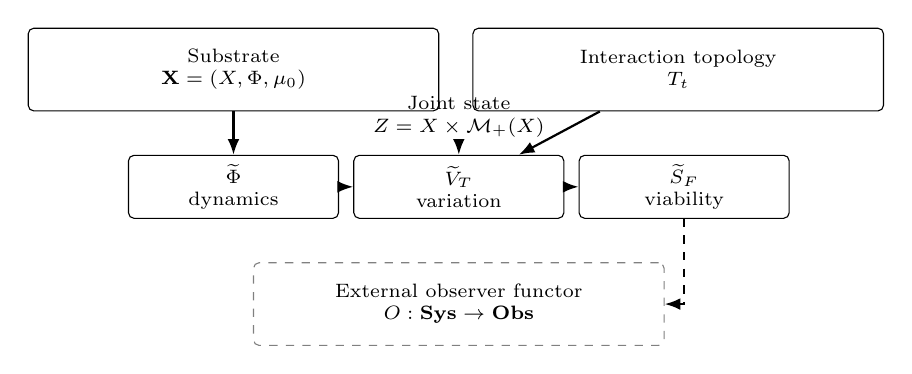
\begin{tikzpicture}[
  font=\scriptsize,
  slot/.style={
    draw,
    rounded corners=2pt,
    align=center,
    minimum width=0.43\columnwidth,
    minimum height=1.05cm,
    inner sep=3pt
  },
  op/.style={
    draw,
    rounded corners=2pt,
    align=center,
    minimum width=0.22\columnwidth,
    minimum height=0.8cm,
    inner sep=2pt
  },
  arrow/.style={-{Latex[length=2mm]},thick}
]
\node[slot] (substrate) {Substrate\\$\X=(X,\Phi,\mu_0)$};
\node[slot, right=0.42cm of substrate] (topology) {Interaction topology\\$T_t$};
\node[op, below=0.55cm of substrate] (phi) {$\widetilde{\Phi}$\\dynamics};
\node[op, right=0.18cm of phi] (var) {$\widetilde V_T$\\variation};
\node[op, right=0.18cm of var] (viab) {$\widetilde S_F$\\viability};
\node[slot, below=0.55cm of var, draw=gray, dashed] (observer) {External observer functor\\$O : \mathbf{Sys} \to \mathbf{Obs}$};
\node[align=center, above=0.1cm of var] (state) {Joint state\\$Z=X\times\Mplus(X)$};

\draw[arrow] (substrate) -- (phi);
\draw[arrow] (topology) -- (var);
\draw[arrow] (phi) -- (var);
\draw[arrow] (var) -- (viab);
\draw[arrow, dashed] (viab) |- (observer);
\draw[arrow] (state) -- (var);
\end{tikzpicture}
\caption{The 4-tuple system $\mathcal{S}=(\X,V,F,T)$ with its external
observer functor (drawn dashed because it is outside the system). The
substrate supplies state and dynamics; interaction topology mediates
variation; viability filters the resulting population measure. The
observer $O : \mathbf{Sys} \to \mathbf{Obs}$ acts on trajectories,
external to the tick rule.}
\label{fig:four-slot}
\end{figure}

\begin{implnote}[Computational implication]
The product structure is deliberate: each slot has its own typing and can be
swapped without rewriting the others. In \S\ref{sec:parallel} we argue that
this same modularity supports a natural GPU mapping in which each slot
becomes a parallel kernel.
\end{implnote}

\subsection{The ambient category $\mathbf{Sys}$}\label{sec:ambient}

The framework commits to a specific ambient category for systems:
$\mathbf{Sys}$ is the \textbf{symmetric monoidal category of
$\mathcal{O}_W$-algebras valued in $\mathbf{Stoch}$}, where $\mathcal{O}_W$
is the operad of wiring diagrams of Vagner, Spivak \&
Lerman~\cite{vagner2015algebras} (with extensions to time-indexed systems
via Schultz \& Spivak~\cite{schultz2020sheaves}) and $\mathbf{Stoch}$ is a
Markov category of measurable spaces and Markov kernels in the sense of
Fritz~\cite{fritz2020synthetic}. Objects of $\mathbf{Sys}$ are
$\mathcal{O}_W$-algebras $A : \mathcal{O}_W \to \mathbf{Stoch}$; morphisms
are $\mathcal{O}_W$-algebra natural transformations; the monoidal product
is inherited from $\mathcal{O}_W$ and coincides with the substrate
composition operator $\boxtimes_\kappa$ of \S\ref{sec:substrates} (the
associativity-up-to-canonical-isomorphism of $\boxtimes_\kappa$ becomes
the SMC structure of $\mathbf{Sys}$).

This choice has three load-bearing properties for the rest of the
framework. First, the typing of the slots and their composition is
operadic-native: $V_T$ construction (\S\ref{sec:vt}) is precisely an
$\mathcal{O}_W$-algebra action. Second, Yau's finite-presentation
theorem~\cite{yau2018operads} for $\mathcal{O}_W$ (eight generators,
twenty-eight relations for the directed case) reduces decomposition
arguments to checking a finite list of cases --- the load-bearing finite
check for the necessity conjecture \textbf{N1}
(\S\ref{sec:conjectures}). Third, the choice is light enough to make the
early theorems tractable: 2-categorical and double-categorical upgrades
are reserved for specific obstructions if they arise but are not
foundational.

A complementary \textbf{interpretive lift} to a sheaf topos is available
via three functorial bridges. The temporal axis is covered by Schultz
\& Spivak~\cite{schultz2020sheaves}, whose temporal type theory provides
a functor from $\mathcal{O}_W$-algebras to sheaves on a base site of
time-windows. The abstract bridge is the classifying topos of
$\mathcal{O}_W$: every operad $\mathcal{O}$ admits a classifying topos
$\mathbf{Sh}(\mathcal{O})$ such that $\mathcal{O}$-algebras in any topos
$\mathcal{T}$ correspond to geometric morphisms $\mathcal{T} \to
\mathbf{Sh}(\mathcal{O})$. The practical bridge is substrate-induced
locality: when the substrate $\X$ carries a natural locality structure
(lattice geometry, particle positions, memory adjacency), that locality
pulls back through the $\mathcal{O}_W$-algebra to a site $\mathcal{B}$ of
substrate patches, and the algebra induces an honest sheaf on
$\mathcal{B}$. The strategy is \emph{prove in the operadic ambient,
interpret in the sheaf topos}. The Aristotelian /
autopoietic~\cite{maturana1980autopoiesis} / free-energy-principle
readings of biology remain available through this lift; they are not
foundational but interpretive layers over the same underlying algebra.

\subsection{The independent observer functor}\label{sec:observer}

An \textbf{observer} is a category-theoretic functor
\[
  O \;:\; \mathbf{Sys} \;\longrightarrow\; \mathbf{Obs},
\]
where $\mathbf{Obs}$ is a category of \emph{observation records} (objects:
measurable spaces of observation traces; morphisms: measurable maps). $O$
sends a system $\mathcal{S}$ to its trajectory-functor
\[
  O(\mathcal{S}) \;:\; \mathbb{N} \;\longrightarrow\; Y,
  \qquad t \;\longmapsto\; O_t\!\big((x_s,\mu_s)_{s\le t}\big),
\]
which assigns to each tick $t$ an observation $O_t \in Y$ computed from a
window of trajectory. Stateful observers are accommodated by allowing $O$
to carry an observer state $a_t \in A_O$ that updates as
$(o_t, a_{t+1}) = O_s\big((x,\mu)_{t-w:t+1}, a_t\big)$; the observer state
records archives, descriptor maps, learned embeddings, or saturation
criteria as appropriate.

\textbf{Independence} is now a property of the morphism, not of the
system: $O$ is independent of $\mathcal{S}$ when it factors through the
trajectory functor of $\mathcal{S}$ rather than through any of the slots
$V, F, T$. Equivalently, $O$ does not appear on the right-hand side of
the iteration rule
$\widetilde S_F \circ \widetilde V_T \circ \widetilde \Phi$. The default
observer is independent. Some systems feed observer output back into
$V$ via archive state (novelty-search-style adaptive variation); this is
modelled as a \emph{second} observer $O'$ whose output is post-composed
onto $V$'s parameter space via the $\rho$-coupling construction of
\S\ref{sec:variation}, not as $O$ being placed inside the tick rule. The
independence of the primary observer is structural; whether one wires
auxiliary observers back into variation is a modelling choice.

Three observer families recur in practice:
\textbf{density-distance observers} (novelty search,
Quality-Diversity~\cite{lehman2011novelty,faldor2024leniaqd}), which
score a window of trajectory by a divergence $D(\mu_{[t-w,t]} \,\Vert\,
\mu_{\mathrm{ref}})$;
\textbf{foundation-model embedding observers}, which embed trajectories
with a foundation model and score in embedding space, as in
ASAL~\cite{kumar2024asal} and OMNI-EPIC~\cite{faldor2024omniepic};
and \textbf{information-theoretic observers}, including mutual
information, transfer entropy~\cite{schreiber2000measuring}, and
integrated-information quantities. Conjecture C3 (now restated under the
pivot framing, see \S\ref{sec:conjectures}) proposes that all three
families are instances of a single divergence-functional schema viewed
through the observer functor.

A trajectory $(x_t,\mu_t)_{t \geq 0}$ of $\mathcal{S}$ is \emph{alive
with respect to observer $O$} when $O(\mathcal{S})$ reports the
structural conditions of $\mathbf{LifeCat}$ membership
(\S\ref{sec:vitality}). The observer is the witness, not the source, of
aliveness; the structural conditions are intrinsic to $\mathcal{S}$.

\subsection{Recursive level structure}\label{sec:recursive-levels}

The framework's hierarchy of organisation is defined \textbf{recursively},
with no a-priori taxonomy of levels by human categories (substrate,
entity, population, meta). Those labels become emergent descriptions of
what the recursion produces in particular systems.

\paragraph{Base case (level 0).} $\Phi$ explores the substrate state
space $X$. The \emph{level-0 entities} are the persistent patterns
produced by $\Phi$ alone: $(S, \pi)$ pairs satisfying the information-
closure condition E1 (Definition~\ref{def:entity}) with variation given
by identity (they persist by $\Phi$, not by any separate $V$ acting on
them).

\paragraph{Recursive case (level $n \geq 1$).} The system reaches level
$n$ iff:

\begin{enumerate}[leftmargin=2em,itemsep=2pt]
  \item \emph{Lower-level search continues:} the system reaches level
    $n - 1$.
  \item \emph{Search acts on level-$(n{-}1)$ entities:} there exists a
    pair $(V_n, F_n)$ acting on the level-$(n{-}1)$ entities such that
    $V_n$ is non-trivial (Definition~\ref{def:vnontriv}), $F_n$ is
    non-trivial (Definition~\ref{def:fnontriv}), and the iteration
    retains \emph{discriminative capacity} at level $n$
    (Definition~\ref{def:disc-cap}).
\end{enumerate}

The \emph{level-$n$ entities} are the persistent patterns at level $n$
--- $(S, \pi)$ pairs satisfying E1 under the $(V_n, F_n)$-induced
dynamic.

The recursion bottoms out at level 0 and ascends through the system's
hierarchical structure. The depth $k$ of the recursion for a given
system is the deepest level at which the recursive case fires. Under the
operadic ambient (\S\ref{sec:ambient}), level $n$ corresponds to
arity-$n$ compositions of $\mathcal{O}_W$ --- the level count is not an
additional axiom but falls out of the ambient category's structure.

\paragraph{Where modeler choice still enters.} The recursive level
structure is structural, but entity-detection at each step depends on
the scale projection $\pi$ (Definition~\ref{def:entity}), which is a
modeler choice. Different reasonable $\pi$ choices typically give the
same level count $k$ but may disagree on which entities exist at each
level. The same modeler-dependence applies to horizontal composition
(\S\ref{sec:horizontal}): whether two physically-coupled subsystems
read as a single entity, a horizontal $\boxtimes_\kappa$ composition, or
a vertical composite depends on $\pi$. The framework's discipline is
that the modeler declares $\pi$; different choices produce internally
coherent but distinct vitality profiles. This is the
Option-A-foundational commitment honoured explicitly: boundaries are
choosable subject to E1, not given from outside.

\subsection{Substrates}\label{sec:substrates}

A \textbf{substrate} is a tuple
\[
  \X \;=\; \big( X, \, \Phi, \, \mu_0 \big),
\]
where $X$ is a measurable space (the \emph{substrate state space}),
$\Phi : X \to X$ (or $\Phi : X \to \Pmeas(X)$ in the stochastic case) is a
measurable \emph{substrate dynamics} map, and $\mu_0 \in \Mplus(X)$ is an
initial measure. Plainly, the substrate is the simulation material plus its
native update rule: the grid and cellular-automaton update, the Flow-Lenia
field and its kernel dynamics, the particle state and its motion law, or the
program space and interpreter dynamics. We deliberately \emph{exclude} a
``neighborhood structure'' from the substrate tuple; the relationship between
the substrate and the interaction topology is treated in \S\ref{sec:topology}.

\topic{\texorpdfstring{Substrate composition operator $\boxtimes$}{Substrate composition operator}}

Real instances are often heterogeneous: a Lenia field coupled to a
meteorological forcing field coupled to a population of LLM agents. A na\"ive
Cartesian product $X_1 \times X_2$ inherits no shared geometry, no shared
time-scale, and no notion of cross-substrate coupling. We therefore introduce
the \textbf{substrate composition operator} $\boxtimes$ in two flavours.

\begin{definition}[Free composition]\label{def:free-composition}
Given substrates $\X_1,\X_2$, their \emph{free composition}
$\X_1 \boxtimes \X_2$ has state space $X_1 \times X_2$, dynamics
$\Phi_1 \times \Phi_2$, and initial measure $\mu_0^{(1)} \otimes \mu_0^{(2)}$.
This recovers the Cartesian product as a degenerate case (no coupling).
\end{definition}

\begin{definition}[Coupled composition]\label{def:coupled-composition}
A \emph{coupling datum} between $\X_1$ and $\X_2$ is a pair of measurable maps
$\kappa = (\kappa_{1\to 2}, \kappa_{2\to 1})$ with
$\kappa_{i\to j} : X_i \to \Param(\Phi_j)$, where $\Param(\Phi_j)$ is a
measurable space of parameters that re-shape the dynamics $\Phi_j$. The
\emph{$\kappa$-coupled composition} $\X_1 \boxtimes_\kappa \X_2$ has state
space $X_1 \times X_2$, dynamics
\[
  \widetilde\Phi(x_1,x_2) \;=\;
  \big(\Phi_1[\kappa_{2\to 1}(x_2)](x_1),\; \Phi_2[\kappa_{1\to 2}(x_1)](x_2)\big),
\]
and initial measure inherited as in Definition~\ref{def:free-composition}.
\end{definition}

\begin{proposition}[Associativity up to canonical isomorphism]
Free composition is symmetric monoidal on the category of substrates and
substrate morphisms; coupled composition is symmetric monoidal on the
category whose morphisms are coupling-respecting maps.
\end{proposition}

The proof reduces to the corresponding statements for the algebra of open
dynamical systems \cite{vagner2015algebras,schultz2020sheaves,myers2021double}:
coupling data are exactly the ``wires''
of a wiring diagram in those formalisms, and our coupling-respecting
morphisms are the morphisms of that wiring-diagram-algebra.

\begin{implnote}[Computational implication]
$\boxtimes_\kappa$ is the formal foundation for ``modular substrates'': the
biological--atmospheric--cultural composite is built as
$(\X_{\mathrm{bio}} \boxtimes_{\kappa_{12}} \X_{\mathrm{atm}}) \boxtimes_{\kappa_{23}} \X_{\mathrm{LLM}}$
rather than as a flat Cartesian product. Each component substrate keeps its
own kernel; coupling kernels are independent code paths.
\end{implnote}

\topic{Computational regimes}

We say a substrate is \emph{lattice-like} if $X = \prod_{p\in L}\Sigma$ for
some discrete lattice $L$ and per-site alphabet $\Sigma$ (cellular automata,
Lenia, NCA), \emph{particle-like} if $X = \bigsqcup_n (\R^d)^n$ (Particle
Lenia, swarms, Avida-with-positions), \emph{graph-like} if $X$ is a function
space on a graph that may itself evolve, or \emph{discrete-program-like} if
elements of $X$ are programs in some instruction set (Avida, LLM-policy
substrates). $\boxtimes_\kappa$ allows arbitrary heterogeneous compositions,
e.g.\ lattice~$\boxtimes_\kappa$~particle.

\subsection{Entities}\label{sec:entities}

The framework requires a precise notion of \textbf{entity}: many
ALife applications have communities of substrate sites (a Lenia blob, a
flock, a colony of Avida programs) acting as a single locus of variation and
selection. We adopt an information-theoretic, substrate-agnostic definition
that generalises the individuality framework of Krakauer \emph{et al.}
\cite{krakauer2020individuality} and
connects cleanly --- but not exclusively --- to the closure-operator
viability machinery of \S\ref{sec:viability}.

The definition has two reader-facing jobs. First, it identifies the part of the
substrate that currently supports the thing we want to call an entity. Second,
it states the scale at which we will describe that thing. A flock may be
supported by many particles but described by a centroid; a program may be
supported by one memory region and described by its raw instruction sequence.

\begin{definition}[Entity]\label{def:entity}
Let $\X=(X,\Phi,\mu_0)$ be a substrate, and let $X = \prod_{p\in P} X_p$ be a
(possibly trivial) decomposition of the state space into per-site factors
indexed by a set $P$ of \emph{substrate sites}. An \emph{entity} at time $t$
is a pair $e = (S, \pi)$ consisting of:
\begin{enumerate}[leftmargin=2em,itemsep=2pt]
  \item a \emph{supporting set} $S \subseteq P$ of substrate sites, and
  \item a \emph{scale projection}
        $\pi : \prod_{p\in S} X_p \to Y_S$
        to a measurable feature space $Y_S$,
\end{enumerate}
such that, with $\mathbf{x}_S^t := (x_p^t)_{p\in S}$ and
$\mathbf{x}_{\bar S}^t := (x_p^t)_{p\notin S}$,

\begin{description}[leftmargin=2em,itemsep=4pt]
  \item[(E1) Persistence (information closure).]
  There exists $\tau \geq 1$ such that
  \[
    I\!\left(\pi(\mathbf{x}_S^{t+\tau});\, \pi(\mathbf{x}_S^{t}) \,\big|\, \mathbf{x}_{\bar S}^{t}\right)
    \;\geq\;
    I\!\left(\pi(\mathbf{x}_S^{t+\tau});\, \mathbf{x}_S^{t}\right) - \varepsilon,
  \]
  for a specified tolerance $\varepsilon \geq 0$. Thus, most information
  predictive of $\pi$'s future is internal to $S$, conditional on the outside.

  \item[(E2) Boundedness.]
  $1 \leq |S|<\infty$ (or $S$ has finite positive measure under a fixed
  reference measure on $P$).

  \item[(E3) Compositionality.]
  Hierarchical entities are admitted: if
  $e_1=(S_1,\pi_1),\dots,e_k=(S_k,\pi_k)$ are entities with disjoint $S_i$,
  then $e^* = (\bigcup S_i,\, (\pi_1,\dots,\pi_k))$ is an entity provided
  (E1) holds at the joint scale.
\end{description}
\end{definition}

The pair $(S,\pi)$ separates \emph{what supports the entity} (the sites $S$)
from \emph{what scale of description we are committing to} (the projection
$\pi$). Trivial $\pi=\mathrm{id}$ recovers raw-state entities (e.g.\ an Avida
program). Non-trivial $\pi$ recovers macroscopic entities such as Lenia
\emph{Orbium} (where $\pi$ might be a centroid-and-mass map) or
particle-system flocks (where $\pi$ might be the empirical centroid and
inertia tensor).

(E1) closely resembles the ``informational closure'' criterion of
Krakauer \emph{et al.} \cite{krakauer2020individuality} and Bertschinger
\emph{et al.} \cite{bertschinger2008autonomy}. It is
\emph{not} identical to the closure-operator characterisation of viable
supporting sets in \S\ref{sec:viability} --- that machinery operates on the
structure of the supporting set $S$ alone, while (E1) operates jointly on
$(S,\pi)$. The relationship is left as a conjecture
(\S\ref{sec:c1}).

The scale projection $\pi$ explicitly anticipates the coarse-graining
structure of causal emergence (\S\ref{sec:emergence}): every entity carries
with it a candidate macroscale at which one may compute effective
information.

\begin{implnote}
Detecting entities reduces to (i) a search over candidate supporting sets $S$
(e.g.\ connected components above a threshold for Lenia, or autopoietic
preimages for Game-of-Life gliders), and (ii) a search over scale projections
$\pi$. Both steps are embarrassingly parallel across candidates; see
\S\ref{sec:parallel}.
\end{implnote}

\subsection{Variation}\label{sec:variation}

A \textbf{variation operator} is a measurable map
\[
  V \;:\; X \times \Theta \;\to\; \Pmeas(X),
\]
where $\Theta$ is a parameter space (mutation rate, recombination
probabilities, gradient step size, prompt-perturbation distribution).
Stochastic, deterministic, and gradient-based variation are unified by
allowing $V$ to be a Markov kernel; deterministic variation is the Dirac case.
In ordinary simulator language, $V$ is the mutation, recombination, rewrite,
or optimisation step that proposes candidate next entities.

Instances span Gaussian/uniform mutation, bit-flip, $k$-point and uniform
recombination, evolution strategies \cite{salimans2017es}, gradient descent
(treated as deterministic $V$), prompt mutation for LLM-policies,
foundation-model-guided variation \cite{lehman2024large}, and Intrinsically
Motivated Goal Exploration Processes \cite{forestier2022imgep}.

A \textbf{variation channel} is a pair $(V_c, \Theta_c)$ identified with one
inheritance lineage (genetic, cultural, etc.). Coupled inheritance channels
require an operation richer than a tensor product. We define a \textbf{channel
composition operator} $\diamond$:

\begin{definition}[Channel composition]
Given channels $V_1$ and $V_2$ that act on substrate components $\X_1$ and
$\X_2$ of a coupled substrate $\X_1\boxtimes_\kappa \X_2$, and a
\emph{coupling rule} $\rho$ specifying how sampling in one channel may
condition sampling in the other (e.g.\ cultural variation may depend on
genetic state \cite{boyd1985culture}), the composed channel
$V_1 \diamond_\rho V_2$ is the kernel
\begin{align*}
  &(V_1 \diamond_\rho V_2)\!\big((x_1,x_2),(\theta_1,\theta_2)\big) \\
  &\quad=\; \int V_1(x_1,\theta_1') \, V_2(x_2,\theta_2') \,
            \rho\big(d\theta_1',d\theta_2'\,\big|\,x_1,x_2,\theta_1,\theta_2\big).
\end{align*}
\end{definition}

Trivial $\rho$ (independent product) recovers tensor-product variation
$V_1 \otimes V_2$ as a special case; non-trivial $\rho$ supports
gene--culture co-evolution \cite{boyd1985culture}, niche construction
\cite{odlingsmee2003niche}, and stigmergic coupling \cite{grasse1959stigmergie}.

\begin{implnote}
$\diamond_\rho$ is implemented as a single fused kernel that emits both
channels' offspring jointly when they are coupled, and as two independent
kernels when they are not --- the same modularity argument as for
$\boxtimes_\kappa$.
\end{implnote}

\topic{Topology-mediated population variation}\label{sec:vt}

The lifted operator $\widetilde V_T$ in \S\ref{sec:framework} requires a
\emph{population-level} variation kernel
$V_T : \Mplus(X) \times X \to \Mplus(X)$, derived from the per-entity
variation operator $V$ of \S\ref{sec:variation} together with the
interaction topology $T_t$ (\S\ref{sec:topology}). Define $V_T$ as follows.
Let $\mathcal{E}_t$ be the entity set induced by $\mu$ at substrate state
$x$ (the entities $e=(S,\pi)$ admitted by Definition~\ref{def:entity}). Let
$T_t$ be a hypergraph on $\mathcal{E}_t$ with hyperedge set $E(T_t)$ and
hyperedge weights $w_e$. For each hyperedge $e \in E(T_t)$ involving
entities $(e_1,\dots,e_r)$, choose a parameter
$\theta_e = g\!\big(e_1,\dots,e_r\big)$ via a measurable rule $g$ (default:
$\theta_e$ depends only on the focal entity, recovering independent
mutation; non-trivial $g$ encodes recombination, prompt-conditioning, etc.).
Then
\[
  V_T(\mu;x) \;=\; \sum_{e \in E(T_t)} w_e \,
                   V\!\big(\,\mathrm{state}(e),\, \theta_e\,\big),
\]
interpreted as a finite positive measure on $X$ (the channel composition
operator $\diamond_\rho$ of \S\ref{sec:variation} extends this to
multi-channel variation under the same construction). When $E(T_t)$ is the
discrete set of singletons $\{\{e_i\}\}$ with unit weights, $V_T$ collapses
to the per-entity push-forward of $V$ along $\mu$. The expression
$\widetilde V_T(x,\mu) = (x, V_T(\mu;x))$ in \S\ref{sec:framework} now
type-checks.

\subsection{Viability}\label{sec:viability}

A \textbf{viability filter} is a measurable map
$F : \Mplus(X) \to \Mplus(X)$ that selects a sub-population of the
post-variation population. It is the rule that says which proposed entities
remain in the run and with what weight. We characterise the principal
proposals in the literature in terms of closure-operator structure on
supporting sets.

\topic{Four formalisms}

\begin{itemize}[leftmargin=1.5em,itemsep=2pt]
  \item \textbf{Markov-blanket viability} \cite{friston2013life,kirchhoff2018blankets}.
    An entity's supporting set is
    required to admit a sparse-coupling decomposition into
    internal/blanket/external states. Caveats apply
    \cite{aguilera2022particular,biehl2021critique}; see \S\ref{sec:fep}.
  \item \textbf{Autopoietic closure} \cite{maturana1980autopoiesis,beer2014glider,beer2015autopoiesis,beer2020origin}.
    The supporting set must be closed under the network of
    constitutive reactions/transitions; e.g.\ a Game-of-Life glider's
    supporting set is closed under the GoL preimage relation restricted to
    the entity's reaction network.
  \item \textbf{RAF set viability} \cite{hordijk2004raf,hordijk2015algorithms}.
    A reaction set $R'$ is a Reflexively Autocatalytic
    Food-generated (RAF) set if every reaction in $R'$ is catalysed by
    something in $R'$ (or in the food set) and every reactant is producible
    from the food set within $R'$.
  \item \textbf{Minimal Criterion Coevolution} \cite{brant2017mcc}; see also
    \cite{lehman2011novelty}. An entity passes the filter iff it
    satisfies a minimal qualifying predicate (e.g.\ ``solves at least one
    maze''), with co-evolutionary feedback supplying the predicate's content.
\end{itemize}

\topic{Closure-operator interpretation}

The four viability formalisms suggest, but do not yet establish, a common
closure-operator interpretation. We therefore treat the unification as
Conjecture~C1 (\S\ref{sec:c1}), with partial supporting evidence presented
there. \textbf{Until C1 is settled, the four formalisms are not in general
substitutable in code:} a simulator that swaps Markov-blanket viability for
autopoietic closure must verify that the substitution preserves the
predicates the rest of the system relies on. The system-description schema
of \S\ref{sec:description} therefore requires the viability formalism to be
named explicitly, not merely as ``$F : \Mplus(X) \to \Mplus(X)$''.

\topic{Hierarchical viability}

Following (E3) of \S\ref{sec:entities}, we propose a \textbf{hierarchical
viability filter} $F^*$ that accepts a composite entity $e^*$ iff each
component entity $e_i$ satisfies its filter \emph{and} the joint scale
projection $(\pi_1,\dots,\pi_k)$ also satisfies a top-level filter. This is
the obvious move; verifying that the four formalisms behave correctly under
hierarchical composition is open (\S\ref{sec:c2}).

\subsection{Interaction Topology}\label{sec:topology}

The \textbf{interaction topology} specifies \emph{who interacts with whom}:
it is a graph (or, more generally, a hypergraph or simplicial complex) on
entities, possibly time-varying. It is not the material geometry itself. A
substrate may be a square lattice, while the interaction topology may be the
graph of gliders that collide, agents that exchange messages, or particles
within a $k$-nearest-neighbour radius.

\topic{Interaction topology vs substrate topology}

Two distinct notions of topology must be kept separate:

\begin{itemize}[leftmargin=1.5em,itemsep=2pt]
  \item \textbf{Substrate topology.} The intrinsic geometry of the substrate
    state space $X$ (e.g.\ the lattice $L$ of a CA; the manifold structure of
    $\R^d$ for particle systems). This is a property of $\X$ in
    \S\ref{sec:substrates} and \emph{does not appear in the substrate
    tuple} --- it is
    whatever geometry the dynamics $\Phi$ already presupposes.
  \item \textbf{Interaction topology.} A causal coupling structure $T$ on
    \emph{entities}: $T$ is a (possibly weighted, possibly directed,
    possibly time-varying) graph
    $T_t \subseteq \mathcal{E}_t \times \mathcal{E}_t$, where
    $\mathcal{E}_t$ is the entity set at time $t$.
\end{itemize}

The two coincide only in homogeneous lattice CA where every entity is one
site. Otherwise they differ --- a Lenia \emph{Orbium} and a meteorological
field couple via a specific spatial overlap relation that is neither the
lattice topology of the CA nor the trivial complete graph on entities.

\topic{Interaction topology definition}

An \textbf{interaction topology} is a measurable family $T = (T_t)_{t\in\N}$
where each $T_t$ is a hypergraph on $\mathcal{E}_t$ together with edge
weights in some semiring $R$ (typically $\R_{\geq 0}$ or $\{0,1\}$).
Instances include lattice neighbourhoods, range-based interactions on $\R^d$
($k$NN, $\varepsilon$-ball), social graphs (sampled or fixed), pairwise game
graphs (donor--recipient pairings as in \cite{vallinder2024cultural}), and
stigmergic indirect-coupling topologies in which interactions pass through
the substrate rather than directly between entities \cite{grasse1959stigmergie}.

\topic{Multi-regime topologies}\label{sec:multi-regime-topologies}

When several coupling regimes coexist (a colony with both within-colony
chemical signalling and between-colony pheromone trails), $T$ is no longer a
single graph but a \textbf{layered multiplex}:
$T = \bigsqcup_\ell T^{(\ell)}$ with non-negative layer weights
$(\alpha_\ell)$ summing to one (so the total interaction load per tick is
preserved). Variation $V_T$ on a multiplex topology is the corresponding
\emph{mixture} of layer kernels,
$V_T(\mu;x) = \sum_\ell \alpha_\ell\, V^{(\ell)}_{T^{(\ell)}}(\mu;x)$, when
channels are independent, or the $\diamond_\rho$-composition
(cf.\ \S\ref{sec:variation}) when they are not. The mixture form
guarantees that $V_T(\mu;x) \in \Mplus(X)$ whenever each layer kernel is.

\subsection{Non-triviality}\label{sec:nontriviality}

The recursive level structure of \S\ref{sec:recursive-levels} uses
``non-trivial $V$'' and ``non-trivial $F$'' in its inductive step. The
following definitions tighten the terms.

\begin{definition}[Non-trivial variation operator]\label{def:vnontriv}
A variation operator $V_n : E_{n-1} \times \Theta \to \Pmeas(E_{n-1})$
on the space of level-$(n{-}1)$ entities is \emph{non-trivial} iff there
exists $e \in E_{n-1}$ and $\theta \in \Theta$ such that
$V_n(e, \theta) \neq \delta_e$. A stronger condition, \emph{diversifying},
holds when $V_n(e, \theta)$ has positive Shannon entropy for some
$(e, \theta)$.
\end{definition}

In plain terms: $V_n$ is non-trivial when some input produces some
output that differs from the input. The identity map (every entity
reproduces itself exactly) is the only trivial case. Most operationally
interesting variation operators are diversifying.

\begin{definition}[Non-trivial viability filter]\label{def:fnontriv}
A viability filter $F_n : \Mplus(E_{n-1}) \to \Mplus(E_{n-1})$ is
\emph{non-trivial} iff it is not a scalar multiple of the identity:
there exist entities $e_1, e_2 \in E_{n-1}$ such that
\[
  \frac{F_n(\delta_{e_1})(\{e_1\})}{F_n(\delta_{e_2})(\{e_2\})} \;\neq\; 1.
\]
\end{definition}

In plain terms: $F_n$ is non-trivial iff it differentially retains
different entities. A filter that scales every entity's retention by the
same factor (e.g.\ a fixed death rate applied uniformly) is trivial in
this sense --- it changes total mass but not relative composition. A
filter that retains some entities preferentially is non-trivial.

\begin{definition}[Discriminative capacity at level $n$]\label{def:disc-cap}
A level-$n$ iteration $(V_n, F_n)$ has \emph{discriminative capacity at
level $n$} iff, for any candidate entity $e^\ast \in E_{n-1}$ that is
strictly fitter than the current population --- meaning
$F_n(\delta_{e^\ast})(\{e^\ast\}) / F_n(\delta_e)(\{e\}) > 1$ for all
$e$ in the current population --- the iteration $V_n \circ F_n$ applied
to the population augmented by $\epsilon\,\delta_{e^\ast}$ gives
$e^\ast$ a strictly increasing share of the population mass over time,
for all sufficiently small $\epsilon > 0$.
\end{definition}

In plain terms: a fitter mutant injected into the population grows in
relative frequency. The condition is observable via a perturbation
experiment: drop a known-fitter mutant into the simulation, run forward,
check that its share grows. This is the operational condition that
distinguishes a converged-but-still-search-active GA (which would
amplify a strictly fitter mutant if one appeared) from a frozen-in-time
snapshot (which would not). The condition replaces an earlier
``not at a fixed point'' formulation that incorrectly excluded
homeostatic systems.

These three definitions cleanly exclude the cases the framework needs
to exclude. A hurricane has trivial $V$ at level 1 (no variation
operator proposes new hurricane variants) and trivial $F$ at level 1
(no filter selects among them); the recursion in
\S\ref{sec:recursive-levels} halts at level 0 by these conditions, not
by hand-waving.

\subsection{Vitality profile and $\mathbf{LifeCat}$ membership}\label{sec:vitality}

The framework's central predicate ---  ``the system--observer pair
$(\mathcal{S}, O)$ is alive'' --- is reported as a structured
measurement on $\mathcal{S}$.

\begin{definition}[Vitality profile]\label{def:vitality}
The \emph{vitality profile} of a system $\mathcal{S}$ relative to a
choice of scale projections at each level is the pair
\[
  (k, \boldsymbol{\sigma}) \;\in\; \N \times [0,1]^k,
\]
where $k$ is the search-hierarchy depth of $\mathcal{S}$ defined
recursively per \S\ref{sec:recursive-levels} and $\boldsymbol{\sigma} =
(\sigma_1, \ldots, \sigma_k)$ is the level-indexed \emph{self-reference
vector}: at each level $i \leq k$,
\[
  \sigma_i \;:=\; \frac{T\!\big(\mathrm{state}_i^t \,\to\, F_i^{t+1} \;\big|\; \mathrm{population}_i^t\big)}{T_{\max}}
\]
is the conditional transfer entropy from the system's level-$i$ state
to the level-$i$ filter's output, given the level-$i$ population,
normalised by its theoretical maximum.
\end{definition}

In plain terms: $k$ measures how deep the system's nested
variation-and-selection hierarchy reaches, and $\sigma_i$ measures
whether the viability filter at level $i$ depends on the system's own
state beyond the current population. $\sigma_i = 1$ corresponds to
fully autopoietic / coevolutionary self-shaping at level $i$;
$\sigma_i = 0$ corresponds to an externally-fixed objective at level
$i$. The pair $(k, \boldsymbol{\sigma})$ is the framework's
substrate-agnostic structural measurement of life-likeness.

\begin{definition}[$\mathbf{LifeCat}$ membership]\label{def:lifecat}
A system--observer pair $(\mathcal{S}, O)$ is a member of
$\mathbf{LifeCat}$ iff its vitality profile $(k, \boldsymbol{\sigma})$
satisfies:
\begin{enumerate}[leftmargin=2em,itemsep=2pt]
  \item \emph{Emergence:} $\sup_\Pi \mathrm{CE}(M(\mathcal{S}), \Pi) > 0$
    (Definition~\ref{def:CE} below).
  \item \emph{Entity persistence:} there is an entity
    $e = (S, \pi)$ whose support remains non-empty across a window of
    the trajectory, with positive $F$-weight.
  \item \emph{Search-active at level $k \geq 1$:} the recursive level
    structure (Defs.~\ref{def:vnontriv}--\ref{def:disc-cap}) reaches
    depth at least one.
\end{enumerate}
\end{definition}

The membership predicate is binary (a pair is in $\mathbf{LifeCat}$
or it is not, depending on whether $k \geq 1$). The full vitality
profile is reported as an \emph{attribute} of each member, capturing
the structural complexity that biology distinguishes via the cluster
of properties traditionally associated with ``how alive'' a thing is.

\paragraph{Where the framework's content lives.} Conditions~1 and~2
are intrinsic to $\mathcal{S}$. The level-$k$ condition is intrinsic.
The self-reference vector $\boldsymbol{\sigma}$ is intrinsic. The
observer functor $O$ does not enter the membership predicate; it
\emph{reports} the profile but does not constitute it. The
independence of the observer (\S\ref{sec:observer}) is what makes
``life'' a well-defined structural property of $\mathcal{S}$ rather
than a perspective-dependent label.

\paragraph{Worked vitality profiles.} The predicate gives principled
verdicts across the range of cases the framework needs to handle:

\begin{center}
\renewcommand{\arraystretch}{1.15}
\setlength{\tabcolsep}{4pt}
\scriptsize
\begin{tabular}{@{}p{0.35\columnwidth} p{0.30\columnwidth} c@{}}
\hline
\textbf{System} & \textbf{Vitality profile} & \textbf{In $\mathbf{LifeCat}$?} \\
\hline
Hurricane                                    & $(0, ())$                       & No  \\
Chaotic map, no entity                       & $(0, ())$                       & No  \\
Plain Game-of-Life glider, no $V$            & $(0, ())$                       & No  \\
Standard converged GA                        & $(1, (0))$                      & Yes \\
Bacteria in fixed nutrient bath              & $(1, (1))$                      & Yes \\
Frequency-dependent GA                       & $(1, (1))$                      & Yes \\
Active Tierra arms race                      & $(2, (1, 1))$                   & Yes \\
Stabilised Tierra                            & $(2, (1, 0))$                   & Yes \\
HeLa cells in lab culture                    & $(2, (1, \approx 0.4))$         & Yes \\
Wild bacterial ecosystem                     & $(2, (1, 1))$                   & Yes \\
Multicellular organism                       & $(3, (1, 1, 1))$                & Yes \\
Human language / cultural evolution          & $(3, (1, 1, 1))$ or deeper       & Yes \\
\hline
\end{tabular}
\end{center}

The framework reads all of the ``yes'' rows as alive in the same
formal sense; the differences in structural complexity are captured
by the full profile $(k, \boldsymbol{\sigma})$, not by binary
membership. A converged GA at $(1, (0))$ and a wild bacterial
ecosystem at $(2, (1, 1))$ are both alive; the bacterial ecosystem is
\emph{more structurally alive} in the precise sense that it reaches a
deeper level with non-zero self-reference at both. The framework's
substrate-agnosticism is operationally cashed out: Tierra in its arms
race phase lands at the same profile as a wild bacterial ecosystem,
which is the operational content of the claim that programmatic life
and biological life are the same theorem in different substrates.

\subsection{Horizontal composition}\label{sec:horizontal}

The recursive level structure of \S\ref{sec:recursive-levels} describes
\textbf{vertical composition}: level-$n$ entities become the substrate for
level-$(n{+}1)$ search, and the recursion climbs the hierarchy. This is
one of two compositional moves the framework needs. The other is
\textbf{horizontal composition} via the substrate-composition operator
$\boxtimes_\kappa$ of Definition~\ref{def:coupled-composition}.

Under the ambient category $\mathbf{Sys}$ (\S\ref{sec:ambient}),
$\boxtimes_\kappa$ is the \emph{monoidal product}: its associativity
up to canonical isomorphism is precisely the SMC structure of
$\mathbf{Sys}$. Horizontal composition combines systems running in
parallel at the same level rather than stacking them into a higher
level.

\paragraph{Effect on vitality profiles.}
Given systems $\mathcal{S}_1$ and $\mathcal{S}_2$ with vitality profiles
$(k_1, \boldsymbol{\sigma}_1)$ and $(k_2, \boldsymbol{\sigma}_2)$ where
$k_1 = k_2 = k$, the horizontal composite $\mathcal{S}_1
\boxtimes_\kappa \mathcal{S}_2$ has depth $k$ (level is preserved). Its
$\boldsymbol{\sigma}$ depends on the coupling structure:

\begin{itemize}[leftmargin=1.5em,itemsep=2pt]
  \item \emph{Trivial $\kappa$} (independent product): composite $\sigma_i
    \approx \max(\sigma_i^{(1)}, \sigma_i^{(2)})$. No new self-reference
    is created.
  \item \emph{One-way coupling} ($\kappa_{1 \to 2}$ non-trivial,
    $\kappa_{2 \to 1}$ trivial): $\mathcal{S}_2$'s effective $\sigma_i$
    rises by the dependence on $\mathcal{S}_1$; $\mathcal{S}_1$'s is
    unchanged.
  \item \emph{Mutual coupling}: $\sigma_i$ for the composite can
    strictly exceed either component's. \textbf{This is the case where
    horizontal composition manufactures self-reference} that was not
    present in either component on its own.
\end{itemize}

The mutual-coupling case is the operationally interesting one. It is
the formal mechanism behind coevolution: a host lineage with
$\sigma_2^{(1)} = 0$ under Darwinian selection from a fixed environment
horizontally composed with a parasite lineage with $\sigma_2^{(2)} = 0$
via mutual $\kappa$ jumps to a composite with $\sigma_2 = 1$. Tierra
during the arms race, predator--prey ecologies, host--parasite
biology, and bilingual speech communities all instantiate this
mechanism. The historical observation that ``coevolution feels
open-ended'' becomes the formal statement that mutual horizontal
coupling generates $\sigma$ uplift.

\paragraph{Examples across substrates.} A non-exhaustive list of cases
worth keeping in mind:

\begin{itemize}[leftmargin=1.5em,itemsep=2pt]
  \item \emph{Symbiosis (lichen).} Alga $(1, (1))$ + fungus $(1, (1))$,
    horizontally composed via mutualistic metabolic coupling. The
    composite is at level 1 but is operationally a single entity in
    many readings.
  \item \emph{Coevolutionary populations (Tierra arms race).} Host
    lineage and parasite lineage at level 2, horizontally composed via
    mutual exploit/resist coupling. Composite has $\sigma_2 = 1$
    manufactured by the coupling.
  \item \emph{Coupled organs.} Heart + lungs in a vertebrate, both at
    organ-system level, composed via circulatory $\kappa$.
  \item \emph{Endosymbiosis.} Historically, ancestral bacterium
    $\boxtimes$ archaeon at level 1, fused so tightly the composite
    now reads as a single level-1 entity (the eukaryotic cell).
  \item \emph{Bilingual speech communities.} Two languages at level 2,
    horizontally composed via shared speakers, code-switching, and
    loanword traffic.
  \item \emph{Hybrid biological--computational systems.} A bacterium
    horizontally composed with a foundation-model agent observing and
    acting on it; cross-substrate coupling.
\end{itemize}

The two compositions can be applied in any order. Real life-forms
typically exhibit both: a multicellular organism is vertically composed
(cells stacked into tissues into organs) and horizontally coupled to
its microbiome, environment, and conspecifics.

\subsection{Cross-system comparison}\label{sec:comparison}

A natural question once $(k, \boldsymbol{\sigma})$ is defined: when can
we say one system is ``more alive'' than another? Two systems will, in
general, have different state spaces and different probability measures,
so the floating-point values of $\sigma_i$ are not literally on the
same scale across systems. The framework handles cross-substrate
comparison with three distinct operations, each appropriate in
different contexts.

\paragraph{Structural equivalence in $\mathbf{LifeCat}$.} Two systems
with the same $k$ and componentwise-equal $\boldsymbol{\sigma}$ (within
estimator tolerance) are \emph{structurally equivalent} as objects of
$\mathbf{LifeCat}$. They have the same categorical shape --- the same
depth of search hierarchy, with the same self-reference at each level
--- regardless of substrate differences. A Tierra arms race at
$(2, (1, 1))$ and a wild bacterial ecosystem at $(2, (1, 1))$ are
structurally equivalent in this sense. Structural equivalence is
necessary but not sufficient for operational equivalence; two
structurally-equivalent systems can still differ under any particular
observer.

\paragraph{Partial order on profiles.} Define
\[
  (k_1, \boldsymbol{\sigma}_1) \;\preceq\; (k_2, \boldsymbol{\sigma}_2)
  \;\iff\; k_1 \leq k_2 \text{ and } \forall i \leq k_1,\;
  \sigma_{1, i} \leq \sigma_{2, i}.
\]
System 2 is ``at least as life-like'' as System 1 iff it dominates in
every component. Most pairs of systems are incomparable in this partial
order, and this is the right answer rather than a bug. A
strong-autopoiesis-but-shallow system $(1, (1.0))$ and a
deep-but-weakly-coupled system $(3, (0.3, 0.3, 0.3))$ are not
ordered by $\preceq$ --- neither dominates the other --- and the
framework's partial order refuses to fabricate an ordering between
them.

\paragraph{Observer-mediated quantitative comparison.} Quantitative
comparison across substrates requires a common observer functor $O$
valid for both systems. Given $\mathcal{S}_1, \mathcal{S}_2$ and $O$,
compute $O$'s output trajectories and compare via a divergence
$D(O(\mathcal{S}_1) \,\Vert\, O(\mathcal{S}_2))$ (KL, Wasserstein, MMD,
or any divergence satisfying C3 in \S\ref{sec:conjectures}). The result
is observer-relative: the same two systems compared under different
observers can produce different orderings, and the framework treats
this as a feature, not a bug. ASAL's CLIP-embedding
observer~\cite{kumar2024asal} is the canonical substrate-independent
observation space in which Lenia, Boids, Tierra, and any
renderable-as-images system become quantitatively comparable.

\paragraph{Reporting discipline.} A framework-conforming comparison
between two systems reports three items: (i) both systems' vitality
profiles, (ii) the partial-order verdict (LT, EQ, GT, or INCOMPARABLE),
and (iii) if a quantitative comparison is needed, the specific
observer $O$ and divergence $D$ used. The discipline forbids cheap
``higher $\sigma$ therefore more alive'' claims when the systems do
not share a measure. The legitimate move is either ``structurally
equivalent,'' or ``incomparable in the partial order,'' or ``ordered
relative to observer $O$ and metric $D$.''

The thermodynamic analogy is apt: $(k, \boldsymbol{\sigma})$ is the
framework's substrate-agnostic ``temperature'' of life; observer-
mediated quantities are the further substrate-specific measurements
(``heat capacity'', ``specific heat''). Two systems at the same
temperature can have different heat capacities; both facts are real,
and the framework's discipline is to keep them straight.

\subsection{Level emergence}\label{sec:le}

The recursive level definition of \S\ref{sec:recursive-levels} is
\emph{static}: given a system, it determines what level the system has
reached. It does not describe how a system at depth $k$ comes to reach
depth $k+1$. But the historical and dynamical reality is that
biological life underwent multiple level transitions --- chemistry
$\to$ cells, cells $\to$ multicellular organisms, organisms $\to$
ecosystems, hominids $\to$ cultures --- and the framework should
describe the mechanism of these transitions, not just the resulting
hierarchy.

Biology calls these \textbf{major evolutionary
transitions}~\cite{maynardsmith1995major,buss1987evolution,west2015majortransitions}.
Eight have been catalogued by Maynard Smith \& Szathm\'ary (replicating
molecules $\to$ compartments $\to$ chromosomes $\to$ DNA + protein
$\to$ eukaryotes $\to$ sexual populations $\to$ multicellular
organisms $\to$ societies $\to$ linguistic societies). These have
not been formalised categorically; the framework does so.

A level transition from depth $k$ to depth $k + 1$ requires the
system to develop a $(V_{k+1}, F_{k+1})$ pair acting on level-$k$
entities. The pair cannot be supplied externally; it must emerge from
the dynamics of level-$k$ entities themselves. Four conditions, drawn
from the cases biology recognises, are the framework's structural
characterisation of the transition. The conditions are themselves
\emph{graded} (each can be partially met), so a system in which the
conditions are partially satisfied is ``on the way to'' a level
transition without having completed one; this is the framework's
content for the ``becoming'' intuition without requiring a separate
continuous quantity.

\begin{namedconjecture}{LE: Level Emergence}
A system $\mathcal{S}$ at vitality profile depth $k$ undergoes a
level transition to depth $k + 1$ over a time window $W$ if and only
if its level-$k$ entities satisfy four conditions over $W$:

\begin{enumerate}[leftmargin=2em,itemsep=2pt]
  \item \emph{Persistence.} Level-$k$ entities have lifetimes much
    longer than the substrate's relaxation time. There must be
    something durable to aggregate before aggregation can produce a
    new level.
  \item \emph{Aggregation.} A non-trivial coupling structure
    $\kappa^{(k)}$ on level-$k$ entities (\S\ref{sec:horizontal})
    produces persistent multi-entity patterns. These are the
    \emph{candidate} level-$(k{+}1)$ entities.
  \item \emph{Group variation.} The coupling $\kappa^{(k)}$ varies
    across the population of aggregates; different aggregate types
    are possible and arise with positive frequency. This is the
    precursor to $V_{k+1}$.
  \item \emph{Group selection.} Different aggregate types have
    measurably different persistence rates. This is the precursor to
    $F_{k+1}$.
\end{enumerate}
\end{namedconjecture}

When all four conditions are met over a sufficient time window, the
persistent aggregates become the level-$(k{+}1)$ entities, the
variation among them becomes $V_{k+1}$, the differential selection
becomes $F_{k+1}$, and the system's depth has increased by 1.

\paragraph{Walking through chemistry $\to$ cells $\to$ organisms $\to$
ecosystems.} The four conditions apply uniformly to each transition;
only the starting substrate differs.

\emph{Chemistry $\to$ cells.}
Persistence: autocatalytic chemical reaction networks (RAFs in the
sense of Hordijk \& Steel~\cite{hordijk2004raf,hordijk2015algorithms})
persist in primordial chemistry as level-0 entities.
Aggregation: lipid bilayer membranes form spontaneously and enclose
patches of chemistry; the membrane is $\kappa^{(0)}$.
Group variation: different membrane compositions, different enclosed
reactions, different geometries.
Group selection: proto-cells with internally self-sustaining
chemistry persist; ones whose chemistry collapses do not. Result:
level-1 entities (cells) emerge as a new categorical type.

\emph{Cells $\to$ organisms.}
Persistence: free-living cells reproduce and persist.
Aggregation: cell-cell adhesion molecules link cells into colonies
(Volvox) or true multicellular structures.
Group variation: different patterns of cell adhesion, different
multicellular geometries, different division-of-labour configurations.
Group selection: some multicellular configurations are mechanically
and metabolically stable; others fall apart. Result: level-2 entities
(multicellular organisms) emerge.

\emph{Organisms $\to$ ecosystems.}
Persistence: free-living organisms persist over generations.
Aggregation: organisms develop trophic relationships, mutualisms,
competitive interactions, niche construction~\cite{odlingsmee2003niche};
the coupling $\kappa^{(2)}$ is the food web plus interaction matrix.
Group variation: different community compositions, food-web
topologies, species assemblages.
Group selection: stable communities (cycled nutrients, balanced
trophic levels) persist; collapsed ones don't. Result: level-3
entities (ecosystems) emerge.

The same mechanism reads each transition uniformly; only the
starting-level substrate differs. LE applies in non-biological
substrates as well: Tierra during its arms race underwent the
level-1 $\to$ level-2 transition (individual programs aggregated into
ecological roles); cultural transitions (spoken $\to$ written
language; pre-literate $\to$ literate societies; pre-Internet $\to$
post-Internet communication networks) are predicted by LE; engineered
multi-agent systems can undergo level transitions when stable
coalitions and niches form.

The negative predictions are equally important. Hurricanes do not
undergo level transitions because their level-0 entities do not
satisfy conditions 3 and 4 (no variation among hurricane types, no
differential persistence among aggregates). A converged GA does not
undergo a transition because its level-1 entities do not aggregate
into stable higher-level structures.

\subsection{Emergence}\label{sec:emergence}

This paper uses a single mathematical definition of emergence:
\textbf{Hoel-style causal emergence}, anchored on \textbf{effective
information} \cite{hoel2013macro,hoel2017map,klein2020scales,comolatti2022causal}.
This definition is not derived from the
closure-operator machinery of \S\ref{sec:viability} or the observer-relative
divergence of \S\ref{sec:observer};
instead, the relationship between those components and causal emergence is
posed as an open problem.

\topic{Effective information}

Let $M = (X,P)$ be a discrete-time, finite-state Markovian system on state
space $X$ with transition matrix $P$,
$P_{ij} = \Pr[x^{t+1}=j \mid x^t=i]$. Let $\Hmax$ denote the uniform
distribution over $X$ (the \textbf{intervention distribution}: each cause is
intervened upon equiprobably, \`a la Pearl).

\begin{definition}[Effective information]
The \emph{effective information} of $M$ is
\[
  \EI(M) \;:=\; I_{\Hmax}\!\big(X^t \,;\, X^{t+1}\big)
  \;=\; \frac{1}{|X|}\sum_{i\in X}
        D_{\KL}\!\big(P_{i,\cdot} \,\big\Vert\, \bar P_{\cdot}\big),
\]
where $\bar P_\cdot = |X|^{-1}\sum_i P_{i,\cdot}$ is the marginal effect
distribution under uniform interventions. Equivalently,
$\EI(M)= \mathbf{H}(\bar P_\cdot) - |X|^{-1}\sum_i \mathbf{H}(P_{i,\cdot})$,
the difference between effect-distribution entropy and average row entropy.
$\EI$ admits a decomposition into determinism (low row-entropy) and
non-degeneracy (broad effect distribution); see \cite{hoel2013macro}.
\end{definition}

\topic{Causal emergence}

Let $\Pi : X \twoheadrightarrow X_{\Pi}$ be a \textbf{coarse-graining} (a
measurable partition of $X$ into macrostates, with $X_{\Pi}$ denoting the
quotient set), inducing a macroscale Markov chain
$M^{\Pi} = (X_{\Pi}, P^{\Pi})$ where $P^{\Pi}$ is the lifted transition
matrix obtained by averaging micro-transitions weighted by a macro-state
distribution (see \cite{klein2020scales} for the canonical choice).

\begin{definition}[Causal emergence]\label{def:CE}
The \emph{causal emergence} of $M$ at coarse-graining $\Pi$ is
\[
  \CE(M,\Pi) \;:=\; \EI(M^{\Pi}) - \EI(M).
\]
The system $M$ is \emph{causally emergent} iff
\[
  \sup_{\Pi}\; \CE(M,\Pi) \;>\; 0,
\]
i.e.\ there exists a coarse-graining at which the effective information
strictly exceeds that of the microscale.
\end{definition}

\topic{Emergence of substrate-agnostic systems}

For a system $\mathcal{S}$ in the sense of \S\ref{sec:framework}, write
$M(\mathcal{S})$ for the Markov chain on the joint state space
$Z = X \times \Mplus(X)$ induced by the composite update rule
$\widetilde S_{F} \circ \widetilde V_{T} \circ \widetilde\Phi$. (For
substrate-as-population paradigms in which $\mu$ is implicit in $x$,
$M(\mathcal{S})$ reduces to a chain on $X$.) We say $\mathcal{S}$
\emph{exhibits causal emergence at scale $\Pi$} iff
$\CE(M(\mathcal{S}),\Pi) > 0$, and that $\mathcal{S}$ \emph{is causally
emergent} iff this holds for some $\Pi$, i.e.\ if
$\sup_{\Pi}\CE(M(\mathcal{S}),\Pi) > 0$ (Definition~\ref{def:CE}).

This definition is by construction:

\begin{itemize}[leftmargin=1.5em,itemsep=2pt]
  \item \textbf{Intrinsic.} $\EI$ is computed from the transition matrix; no
    external observer enters its definition. (Contrast
    \S\ref{sec:observer}.)
  \item \textbf{Coarse-graining-based.} The macroscale is a partition $\Pi$
    of $Z$; not a closure condition on supporting sets. (Contrast
    \S\ref{sec:viability}.)
  \item \textbf{Non-trivial.} Whether $\sup_\Pi \CE>0$ holds for given
    $\mathcal{S}$ is a non-trivial property requiring construction of $\Pi$.
    (See \S\ref{sec:op1} for the open problem.)
\end{itemize}

\topic{Extensions and known limitations}

\textbf{$\Phi$ID-based emergence} \cite{rosas2020reconciling,mediano2022parts}
replaces partition-based coarse-grainings with
arbitrary supervenient features $V_t = f(X_t)$, defined causally emergent iff
$V$ has unique predictive information about $X^{t+1}$ that no microscopic
component has. This is feature-agnostic but methodologically more demanding.

\textbf{Comolatti and Hoel} \cite{comolatti2022causal} show that causal emergence is widespread
across causation measures (over a dozen popular formalisms): emergence is
not an artefact of using $\EI$ specifically.

\textbf{Limitations.} The intervention distribution $\Hmax$ is conventional,
not unique; results are sensitive to the choice \cite{dewhurst2021causal}. Sup-over-$\Pi$
is only computable for small $|X|$; tractable algorithmic relaxations exist
\cite{klein2020scales,griebenow2019scale} but do not exhaust the supremum.

\begin{implnote}
$\EI$ is a per-Markov-chain reduction; it composes with the population-level
$\mu_t$ but does not parallelise across the population --- it is computed
once per chain, after $\Phi,V,F$ have produced $P$. Coarse-graining search
is itself parallel: candidate partitions can be evaluated independently.
\end{implnote}

\subsection{Evolution, Culture, and Active-Inference Models}

\topic{Two channels, transmission, niche construction}

A standard cultural-and-genetic system is
\[
  \mathcal{S} \;=\; \big(\,\X_g \boxtimes_\kappa \X_c, \;\; V_g \diamond_\rho V_c, \;\; F, \;\; T, \;\; O\,\big)
\]
where $\X_g$ carries the genetic state, $\X_c$ the cultural state, $\kappa$
encodes how genetic state shapes cultural transmission and vice versa
(gene--culture co-evolution \cite{boyd1985culture}), and the
niche-construction map of \cite{odlingsmee2003niche} is
implemented as a coupling kernel from population state to environmental
sub-substrate. The Donor Game with LLM agents \cite{vallinder2024cultural} is
the discrete instance: $\X_c$ is the prompt-conditioned policy state, $V_c$
is prompt mutation, $T_t$ is the random donor--recipient pairing, $F$ is
fitness-proportional reseeding.

\topic{The free energy principle as a descriptive lens}\label{sec:fep}

We treat the FEP \cite{friston2013life,kirchhoff2018blankets} as a
\textbf{descriptive lens} rather than a derivation: when a system
$\mathcal{S}$ admits a Markov-blanket decomposition that is preserved under
$\Phi$, then internal-state dynamics can be \emph{parameterised} as
variational free-energy minimisation. We do not claim this decomposition is
universal; technical critiques \cite{aguilera2022particular,biehl2021critique}
show that sparse coupling
does not imply Markov-blanket structure in general, and Friston's reply
\cite{friston2022reply} sharpens but does not resolve the
challenge. The FEP is a useful \emph{parameterisation} of viability and
observer slots when applicable; it is not a general theorem of
substrate-agnostic systems. Morphogenesis-as-Bayesian-inference
\cite{kuchling2020morphogenesis} is the canonical biological application.

\subsection{Representative Model Instantiations}\label{sec:instances}

\begin{itemize}[leftmargin=1.5em,itemsep=3pt]
  \item \textbf{Lenia} \cite{chan2019lenia}. $X = [0,1]^L$ on a 2D toroidal
    lattice $L$, $\Phi$ a
    kernel-convolution-and-growth update.
  \item \textbf{Flow-Lenia} \cite{plantec2023flowlenia,plantec2025flowlenia}.
    Adds local mass conservation and parameter localisation, enabling
    multi-species cohabitation.
  \item \textbf{Particle Lenia} \cite{mordvintsev2022particle}.
    Energy-based Lagrangian particle reformulation.
  \item \textbf{Neural Cellular Automata} \cite{mordvintsev2020nca}. $\Phi$ is a small neural
    network applied per-cell.
  \item \textbf{Differentiable Logic CA} \cite{miotti2025dlca}, building on
    differentiable logic gate networks \cite{petersen2022logic,petersen2024convlogic}.
    Discrete-state CA with differentiable training via logic-gate softmaxes.
  \item \textbf{Particle / swarm.} Boids, Particle Life. Particle-like
    substrate; interaction topology a $k$-NN or $\varepsilon$-ball.
  \item \textbf{Avida} \cite{lenski2003origin}; original system
    \cite{adami1994avida}.
    Discrete-program substrate.
  \item \textbf{LLM-policy substrate.} Prompt-conditioned policies as
    elements of $X$; $V$ is prompt mutation or LLM-mediated re-writing
    \cite{vallinder2024cultural,lehman2024large}.
\end{itemize}

\begin{table*}[!t]
\caption{Default slot choices for canonical substrate families.}
\label{tab:defaults}
\centering
\renewcommand{\arraystretch}{1.15}
\setlength{\tabcolsep}{3pt}
\scriptsize
\begin{tabular}{@{}p{0.13\textwidth} p{0.205\textwidth} p{0.19\textwidth} p{0.19\textwidth} p{0.19\textwidth}@{}}
\hline
\textbf{Slot} & \textbf{Lattice-like} & \textbf{Particle-like} & \textbf{Graph-like} & \textbf{Program-like} \\
\hline
$\pi$ (entity scale) &
  connected component above threshold $\to$ centroid $+$ mass &
  flock identifier $\to$ centroid $+$ inertia tensor &
  community identifier $\to$ membership vector &
  $\pi=\mathrm{id}$ (raw program) \\
$V$ default &
  parameter-localised Gaussian on kernel weights &
  Gaussian on per-particle parameters &
  edge rewiring $+$ vertex resampling &
  bit-flip $+$ instruction insertion \\
$F$ default &
  autopoietic closure on the local reaction network &
  spatial-cohesion threshold (cluster persists $\geq \tau$ ticks) &
  RAF detection on edge-catalysis graph &
  MCC predicate (executes a non-trivial program) \\
$T$ default &
  Moore neighbourhood on $L$ &
  $k$-NN on positions &
  the underlying graph itself &
  trivial / topology supplied by interaction protocol \\
$O$ default &
  $\Omega$ metric on attractors &
  density-distance archive on $\R^{d}$ &
  graph-level invariants $+$ embedding novelty &
  fitness $+$ FM-embedding novelty \\
Window &
  $w \approx \tau_{\mathrm{relax}}$ &
  $w \approx \tau_{\mathrm{relax}}$ &
  $w \approx \mathrm{diam}(G)$ &
  $w \approx K$ instructions \\
\hline
\end{tabular}
\end{table*}

\topic{Component-Level Instances}\label{sec:components}

\begin{itemize}[leftmargin=1.5em,itemsep=3pt]
  \item \textbf{Variation:} Gaussian/uniform mutation, bit-flip, $k$-point
    recombination, ES \cite{salimans2017es}, gradient descent
    (deterministic $V$), prompt mutation, IMGEP \cite{forestier2022imgep},
    and FM-guided exploration \cite{kumar2024asal,faldor2024omniepic}.
  \item \textbf{Viability:} Markov-blanket viability; autopoietic closure
    \cite{beer2014glider,beer2015autopoiesis,beer2020origin}; RAF detection
    \cite{hordijk2004raf,hordijk2015algorithms}; MCC \cite{brant2017mcc};
    novelty-archive viability \cite{lehman2011novelty}; Quality-Diversity /
    MAP-Elites filters; POET viability \cite{wang2019poet,wang2020enhanced}.
  \item \textbf{Interaction topology:} lattice neighbourhoods; range-based
    on $\R^d$; static social graphs; dynamic pairing graphs (Donor Game
    \cite{vallinder2024cultural}); stigmergic indirect coupling.
  \item \textbf{Observer:} density-distance archives (novelty search);
    CLIP-embedding observers (ASAL \cite{kumar2024asal});
    Hughes--Dennis novelty-and-learnability \cite{hughes2024openendedness};
    $\Omega$ metric \cite{lopezdiaz2025undecidability}.
\end{itemize}

\topic{Default choices for canonical substrate families}\label{sec:defaults}

The framework is permissive but a simulator author needs starting points.
Table~\ref{tab:defaults} covers the four substrate families introduced in
\S\ref{sec:substrates}; deviations should be reported in the
system description (\S\ref{sec:description}).

These are starting points only; an author who departs from them must
specify the alternative explicitly in the description of
\S\ref{sec:description}.

\topic{Worked Composite Example}\label{sec:worked}

We instantiate every typed object of the scaffold for a Flow-Lenia coupled
to an LLM-naming agent. The point is not the system's empirical interest
but to exhibit a fully-specified instance: a simulator author wishing to
implement the framework can follow this template line-for-line and obtain
a typed iteration rule.

\paragraph{Substrate}
$\X = \X_{\mathrm{FL}} \boxtimes_{\kappa} \X_{\mathrm{LLM}}$, where
\begin{itemize}[leftmargin=1.5em,itemsep=2pt]
  \item $\X_{\mathrm{FL}} = \big([0,1]^{L},\; \Phi_{\mathrm{FL}},\;
        \mu_{0}^{\mathrm{FL}}\big)$ with $L = (\mathbb{Z}/H\mathbb{Z})\times(\mathbb{Z}/W\mathbb{Z})$ a
        toroidal lattice and $\Phi_{\mathrm{FL}}$ the Flow-Lenia
        kernel-convolution-and-growth update of
        \cite{plantec2023flowlenia};
  \item $\X_{\mathrm{LLM}} = \big(\Sigma^{*},\; \mathrm{id},\;
        \mu_{0}^{\mathrm{LLM}}\big)$ with $\Sigma^{*}$ the space of token
        sequences and the LLM substrate dynamics taken to be the identity
        (the LLM is queried, not autonomously evolved);
  \item coupling
        $\kappa = (\kappa_{\mathrm{FL}\to\mathrm{LLM}},\,
                    \kappa_{\mathrm{LLM}\to\mathrm{FL}})$ with
        $\kappa_{\mathrm{FL}\to\mathrm{LLM}}(x_{\mathrm{FL}}) =
         \mathrm{render}(x_{\mathrm{FL}})$ (a text-prompt context drawn
        from the rendered frame) and
        $\kappa_{\mathrm{LLM}\to\mathrm{FL}}(x_{\mathrm{LLM}})$ a
        per-creature scalar viability bonus indexed by the entity's
        support $S$ each tick.
\end{itemize}

\paragraph{Entities}
For each connected component $S \subseteq L$ of
$\{p \in L : x^{\mathrm{FL}}_{p} \geq \theta\}$ above mass-threshold
$\theta$, define
\begin{align*}
  \pi_{\mathrm{FL}}\big((x_{p})_{p\in S}\big) \;=\;
  &\Big(\,\tfrac{1}{m}\textstyle\sum_{p\in S} p\, x_{p},\; m\Big),\\
  m \,:=&\, \textstyle\sum_{p\in S} x_{p},
\end{align*}
giving an $\R^{2}\!\times\!\R_{\geq 0}$-valued centroid-and-mass scale
projection. LLM agents are atomic entities: $S$ a singleton, $\pi=\mathrm{id}$.

\paragraph{Variation}
$V = V_{\mathrm{FL}} \diamond_{\rho} V_{\mathrm{LLM}}$ with
\begin{itemize}[leftmargin=1.5em,itemsep=2pt]
  \item $V_{\mathrm{FL}}(x;\theta) = \mathcal{N}(x,\, \sigma^{2} I)$
        applied to the parameter-localised Flow-Lenia kernel weights
        \cite{plantec2025flowlenia};
  \item $V_{\mathrm{LLM}}(x;\theta)$ resamples each token of $x$ with
        probability $p_{\mathrm{rewrite}}$ from the LLM marginal
        $q(\cdot \mid \mathrm{context})$;
  \item $\rho(d\theta'_{\mathrm{LLM}} \mid x_{\mathrm{FL}},
              x_{\mathrm{LLM}}, \theta_{\mathrm{LLM}})$ re-weights the
        token marginals proportionally to the recent naming-success score
        of the named creatures, biasing prompt mutations toward referents
        that paid off in the last $W$ ticks.
\end{itemize}

\paragraph{Viability}
$F = F^{*}$ a hierarchical filter (\S\ref{sec:viability}):
\begin{itemize}[leftmargin=1.5em,itemsep=2pt]
  \item each Flow-Lenia entity $e_{\mathrm{FL}} = (S,\pi_{\mathrm{FL}})$
        passes iff its support $S$ is closed under the local
        mass-conservation reaction network --- autopoietic closure
        \cite{beer2014glider};
  \item each LLM agent passes iff it has successfully named at least one
        Flow-Lenia entity in the last $W$ ticks (MCC predicate
        \cite{brant2017mcc});
  \item $F^{*}$ accepts the joint configuration iff both component filters
        pass and $|\mathcal{E}_{t+1}^{\mathrm{FL}}| \geq 1$ (a non-extinction
        top-level predicate).
\end{itemize}

\paragraph{Interaction topology}
$T_{t} = T_{t}^{(1)} \sqcup T_{t}^{(2)} \sqcup T_{t}^{(3)}$ a three-layer
multiplex with weights $(\alpha_{1},\alpha_{2},\alpha_{3})$:
$T_{t}^{(1)}$ is spatial-overlap on $L$ for Flow-Lenia entities
(hyperedges = pairs whose supports intersect within radius $r$);
$T_{t}^{(2)}$ is uniformly random pairing of LLM judges and namers;
$T_{t}^{(3)}$ is the bipartite stigmergic layer connecting an LLM agent to
each Flow-Lenia entity it has named.

\paragraph{Iteration rule}
The system is the 4-tuple $\mathcal{S} = (\X, V, F^\ast, T)$ with the
iteration
$(x_{t+1},\mu_{t+1}) =
  \big(\widetilde S_{F^{*}} \circ
        \widetilde V_{T_{t}} \circ
        \widetilde\Phi\big)(x_{t},\mu_{t})$
exactly as in \S\ref{sec:framework}.

\paragraph{External observer}
The observer is an external functor
$O = (O_\Omega, O_{\mathrm{CLIP}}) : \mathbf{Sys} \to \mathbf{Obs}$
with window $w = W$:
\begin{itemize}[leftmargin=1.5em,itemsep=2pt]
  \item $O_\Omega$ is the residence-time $\Omega$
        metric~\cite{lopezdiaz2025undecidability} on the time series of
        distinct Flow-Lenia attractors;
  \item $O_{\mathrm{CLIP}}$ is the mean cosine novelty of CLIP
        embeddings of (frame, name) pairs against an archive of size
        $A$.
\end{itemize}
$O$ is independent of $\mathcal{S}$ in the sense of \S\ref{sec:observer}:
it factors through the trajectory functor of $\mathcal{S}$ and does not
appear in the right-hand side of the iteration rule. Whether the
naming-success score from the LLM side is fed back into the variation
$V_{\mathrm{LLM}}$ is handled by the $\rho$-coupling
construction of \S\ref{sec:variation}, not by
placing the observer inside $\mathcal{S}$.

\paragraph{Vitality profile (target)}
The framework predicts the system reaches vitality profile
$(2, (1, 1))$ during active arms-race phases of the coupled dynamics
(if Flow-Lenia and the LLM-naming agent enter a mutual coevolutionary
regime), and profile $(2, (1, \approx 0))$ if the LLM-side dynamics
stabilises. Computing the profile is the subject of an empirical
methodology paper; the algorithm is specified in companion
documentation accompanying this paper (see
\texttt{docs/vitality\_computation.md}).

\paragraph{Emergence assessment (open)}
Whether $\sup_{\Pi}\CE(M(\mathcal{S}),\Pi) > 0$ holds for this system is a
concrete instance of L1 (= renamed OP1; see
\S\ref{sec:op1}).

\medskip

The framework's substrate-agnosticism is visible: every slot can be
ablated independently --- replace $V_{\mathrm{LLM}}$ with random prompts,
swap $F^{*}$ for Markov-blanket viability, collapse the multiplex $T$
to a complete graph, narrow $O$ to $O_{\mathrm{CLIP}}$ alone --- and the
resulting system remains an instance of the framework. The categorical
comparison machinery of \S\ref{sec:comparison} applies to ablations: the
profile $(k, \boldsymbol{\sigma})$ either changes (in which case the
ablation has structural content) or does not (in which case the
ablation is decorative). Cross-substrate comparison with another
framework instance (e.g.\ Tierra at $(2, (1, 1))$) is by the partial
order on profiles plus a chosen observer.

\subsection{Implementation and Reproducibility}\label{sec:parallel}

Implementation is part of the methodology because the framework is intended
to be reproducible as a simulator scaffold, not only interpreted as a
taxonomy. This subsection therefore records the algorithmic control flow,
synchronization boundaries, complexity assumptions, and reporting schema
needed to instantiate $\mathcal{S}$ in software. No source code is required;
the pseudocode records control flow and synchronization points. The five-slot
decomposition is preserved: each slot becomes its own kernel.

\topic{Inputs and conventions}

Let $N$ be the population size of entities; $|X|$ be the substrate state
size (e.g.\ $H\times W$ for a 2D lattice, or $D$ for an $\R^D$ particle
system); $c_\Phi, c_V, c_F$ be the per-call costs of one substrate update,
one variation draw, and one viability evaluation respectively;
$c_{\mathrm{nn}}$ the cost of a neighbourhood lookup or $k$-NN query; and
$P$ the number of parallel workers (SMs $\times$ warp-equivalents in CUDA
terms; XLA threads in JAX terms).

\topic{Per-tick algorithm}

At each tick $t \to t+1$:

\begin{enumerate}[leftmargin=2em,itemsep=4pt]
  \item \textbf{$\Phi$-kernel (substrate dynamics).} For each substrate site
    or particle, apply $\Phi$ in parallel.
    \begin{itemize}[leftmargin=1.2em,itemsep=2pt]
      \item \emph{Lattice / NCA / Lenia / Flow-Lenia:} a local stencil. Each
        thread computes the update for one site, reading from a halo.
        Embarrassingly parallel modulo halo exchange.
      \item \emph{Particle / swarm:} parallel over particles; each thread
        queries its neighbourhood via a spatial-hash or BVH index. $k$-NN
        is the interaction step.
      \item \emph{Discrete-program substrates (Avida-like):} parallel over
        programs; each thread executes one program for $K$ instructions.
    \end{itemize}
  \item \textbf{$T$-kernel (interaction topology lookup).} Build $T_t$ if
    dynamic. Local stencils need no global structure; $k$-NN/$\varepsilon$-ball
    lookups require a spatial index, which itself parallelises in
    $O(\log |X|)$ depth. Social graphs are gather operations indexed by an
    adjacency list.
  \item \textbf{$V$-kernel (variation).} For each entity $i$ in parallel,
    draw mutated offspring. Per-entity variation is embarrassingly parallel;
    recombination requires an additional gather step indexed by mating
    pairs (selected via $T$).
  \item \textbf{$F$-kernel (viability).} For each entity in parallel,
    evaluate viability predicate. Fitness-proportional selection requires a
    parallel prefix sum (scan) over the population --- a $\log N$-depth
    synchronisation barrier.
  \item \textbf{$\mu$-reduction.} Update population measure; for
    mass-conserving substrates (Flow-Lenia) include a global mass reduction
    over the lattice --- another $O(\log |X|)$-depth scan.
  \item \textbf{$O$-kernel (observer).} Optionally: archive update,
    divergence computation, or FM embedding. $k$-NN novelty is all-to-all
    (or approximate-NN) across the archive; FM embedding is an
    embarrassingly parallel batch forward pass.
\end{enumerate}

The scaffold's products $S_F \circ V_T \circ \Phi$ map onto \textbf{kernels
with explicit synchronisation only at boundaries between slots}. Within a
slot, parallelism is per-site (for $\Phi,F$) or per-entity (for $V$,
novelty).

\topic{Single-threaded complexity}

Per tick, ignoring constants:
\begin{align*}
  T_1(N,|X|)=O\big(& |X|c_\Phi + |E_T|c_{\mathrm{nn}} \\
    &+ Nc_V + Nc_F + c_O(N,|X|)\big),
\end{align*}
where $|E_T|$ is the number of edges in $T_t$ (e.g.\ $O(|X|)$ for lattices
with bounded-degree neighbourhoods, $O(Nk)$ for $k$-NN, $O(N^2)$ for
complete pairwise interaction) and $c_O$ depends on observer family.

\topic{Many-threaded complexity}

With $P$ parallel workers, ideal-case (no contention) per-tick cost is
\begin{align*}
  T_P(N,|X|)=O\bigg(&
    \frac{|X|c_\Phi + |E_T|c_{\mathrm{nn}}}{P} \\
    &+ \frac{Nc_V + Nc_F + c_O(N,|X|)}{P} \\
    &+(\log N + \log |X|)c_{\mathrm{sync}}\bigg),
\end{align*}
where the $\log$ terms come from population-level reductions
($\mu$-mass conservation; fitness-proportional selection prefix-sum) and
from spatial-index construction. In the lattice case with
$|E_T|=\Theta(|X|)$ and stencil cost $c_\Phi=\Theta(1)$, this collapses to
$O(|X|/P + N/P + \log|X|)$.

\topic{Communication patterns}

\begin{itemize}[leftmargin=1.5em,itemsep=2pt]
  \item \textbf{Embarrassingly parallel.} Per-site $\Phi$ on a lattice (with
    halo); per-entity $V$ when channels are independent; per-entity $F$ when
    the predicate is local; FM-embedding observers (batch forward).
  \item \textbf{Local stencils.} Lenia/NCA/Flow-Lenia $\Phi$-kernels; halo
    width = kernel radius. Standard CUDA shared-memory stencil pattern.
  \item \textbf{Population-level reductions.} Mass conservation in
    Flow-Lenia ($O(\log|X|)$); fitness-proportional selection prefix sum
    ($O(\log N)$); $\Omega$-metric residence-time reductions.
  \item \textbf{All-to-all.} $k$-NN observers against archive (all current
    entities vs all archive entries); naive $O(NM)$, approximate-NN
    $O(N\log M)$.
  \item \textbf{Gather operations.} Social-graph indexed lookups;
    $T$-mediated mating pair gather. Bandwidth-limited rather than
    compute-limited.
\end{itemize}

\topic{Random-number considerations}

Each parallel worker requires an independent stream. Counter-based RNGs
such as Philox 4$\times$32-10 \cite{salmon2011parallel} are
appropriate: stream $(i,t)$ is a key-counter pair
$((\text{global seed},i),t)$, allowing reproducible per-worker streams
without locks or pre-computation. JAX's \texttt{jax.random.split} API
instantiates exactly this pattern.

\topic{Modularity and code-reuse benefits}

Each of the five slots becomes a separate kernel. Implementations are:

\begin{itemize}[leftmargin=1.5em,itemsep=2pt]
  \item \textbf{Reusable across substrates:} the $V$-kernel for Gaussian
    mutation is identical whether the substrate is Lenia or a Boids swarm;
    only the input shape differs.
  \item \textbf{Reusable across viability formalisms:} Markov-blanket,
    autopoietic, RAF, and MCC viability all type as
    $\Mplus(X)\to\Mplus(X)$; switching between them is a single function
    pointer, not a rewrite.
  \item \textbf{Reusable across observers:} density-distance, FM-embedding,
    and EI-based observers all take a trajectory and return a vector in
    $\R^k$.
\end{itemize}

This is the pragmatic payoff of the abstract slot decomposition.

\topic{System Description}\label{sec:description}

The framework decomposes any emergent system into the 4-tuple
$\mathcal{S} = (\X, V, F, T)$ plus an external observer $O$, with the
vitality profile $(k, \boldsymbol{\sigma})$ as a derived structural
attribute. A description has two parts: the \textbf{system description}
(intrinsic to $\mathcal{S}$) and the \textbf{observation record}
(intrinsic to $O$ and how it is attached). The two compose at run
time; they do not need to be specified together. The items below are
not a gate the system passes; structural items are exhibitable for
any emergent system by construction, observation-record items are
what an external observer adds, and reproducibility metadata is what
an implementer records so others can re-run the simulator.

\paragraph{System description (intrinsic to $\mathcal{S}$).}
\begin{enumerate}[leftmargin=2em,itemsep=2pt]
  \item Substrate $\X=(X,\Phi,\mu_0)$, including any
    $\boxtimes_\kappa$-decomposition (\S\ref{sec:horizontal}) if
    the system is horizontally composed.
  \item Entity definition: scale projection $\pi$ and the
    entity-detection rule satisfying E1.
  \item Variation operator $V$ and any $\diamond_\rho$ couplings.
  \item Viability filter family $F$ (named explicitly:
    Markov-blanket, autopoietic, RAF, MCC, or other); if departing
    from the default of \S\ref{sec:defaults}, justify.
  \item Interaction topology $T$, including any multiplex layers and
    weights $(\alpha_\ell)$.
  \item Iteration order. Default:
    $\widetilde S_F \circ \widetilde V_T \circ \widetilde\Phi$. Any
    deviation is stated explicitly.
  \item Vitality profile $(k, \boldsymbol{\sigma})$ if computed
    (the profile is not part of the input description; it is
    reported once the trajectory has been observed).
\end{enumerate}

\paragraph{Observation record (intrinsic to $O$).}
\begin{enumerate}[leftmargin=2em,itemsep=2pt,start=8]
  \item Observer functor $O : \mathbf{Sys} \to \mathbf{Obs}$,
    family (density-distance, FM-embedding, or
    information-theoretic), window length $w$, and observer state
    variables (archive size, embedding model, reference
    distribution).
  \item Descriptor space, archive update rule, saturation criterion,
    and boundedness test used by $O$.
\end{enumerate}

\paragraph{Reproducibility metadata (intrinsic to the implementation).}
\begin{enumerate}[leftmargin=2em,itemsep=2pt,start=10]
  \item RNG provenance per kernel (counter-based scheme,
    $(\mathrm{seed},\,\mathrm{worker\,id},\,t)$ key triple).
  \item Per-tick wall-clock and theoretical complexity.
  \item Pseudocode or executable specification for initialization,
    tick update, observer-state update, stopping rule, and outputs.
\end{enumerate}

The system description (items 1--7) follows from the system being an
emergent system at all. The observation record (items 8--9) is what
an external observer additionally specifies; an observer can be
swapped without re-deriving the system description. The
reproducibility metadata (items 10--12) is what an implementer
records for replication; it is independent of both the system and
the observer.

\paragraph{Minimal pseudocode}
A description-complete implementation supplies at least the following
control-flow template, specialised to its chosen slots:
\begin{enumerate}[leftmargin=2em,itemsep=2pt]
  \item Initialise $(x_0,\mu_0)$, topology state, observer state $a_0$, and
    RNG keys.
  \item For $t=0,\ldots,T-1$, compute $x'=\Phi(x_t)$ and push $\mu_t$
    forward if entities are explicit.
  \item Build or update $T_t$ and draw the varied population
    $\mu' = V_{T_t}(\mu_t;x')$.
  \item Apply the viability filter $\mu_{t+1}=F(\mu')$ and set
    $x_{t+1}=x'$.
  \item Evaluate $(o_t,a_{t+1})=O_s((x,\mu)_{t-w:t+1},a_t)$, update any
    archive, and test the stopping or saturation criterion.
  \item Return trajectory summaries, observer outputs, archive state, and
    reproducibility metadata.
\end{enumerate}

\paragraph{Comparing implementations}
Two implementations admit slot-wise comparison when they (i) agree on the
typing of each slot (\S\ref{sec:framework}--\S\ref{sec:observer}); (ii)
record values for the structural items, not just slot names; (iii)
preserve the iteration order of item~7 or explicitly declare a variant;
and (iv) specify the entity-detection rule consistently with
Definition~\ref{def:entity}. Comparison does \emph{not} require choice of
the same fitness landscape, observer family, or coarse-graining $\Pi$;
those are user-level choices. It requires only that a comparison across
two implementations be a comparison of choices, not of unstated defaults.

\section{Results}\label{sec:results}

No concrete results are claimed in this paper beyond the definitions
and statements of conjecture (\S\ref{sec:conjectures}). The framework
targets \textbf{L1} (causal emergence of a scaffolded system) as the
first concrete result, with a Game-of-Life-under-Markov-blanket-
viability candidate identified in \texttt{docs/proof\_techniques.md}.
The proof itself will be developed as a focused result paper under
\texttt{docs/papers/}, not in this manuscript. Subsequent result
papers will address S1, N1, CAT1, LE, C1--C3, OP2, and OP3 in turn,
each under its own subdirectory.

Until L1 lands, this section remains empty.

\section{Discussion}\label{sec:discussion}

\subsection{Conjectures and Open Problems}\label{sec:conjectures}

This section consolidates \emph{all} claims in the framework that we
have \emph{not} proven. They are stated as conjectures or open
problems to distinguish them from definitions and established
propositions. The framework's central content is four top-level
conjectures: \textbf{S1} (sufficiency), \textbf{N1} (necessity),
\textbf{CAT1} (characterisation), and \textbf{LE} (level emergence).
Six lemma-level conjectures (\textbf{C1}, \textbf{C2}, \textbf{C3},
\textbf{L1} = renamed \textbf{OP1}, \textbf{OP2}, \textbf{OP3}) are
re-pointed as sub-claims that contribute to N1's machinery. All ten
are unproven; status is tracked in \texttt{RESULTS.md}.

\topic{Top-level: sufficiency}\label{sec:s1}

\begin{namedconjecture}{S1: sufficiency}
There exists a 4-tuple system $\mathcal{S}$ and an external observer
functor $O$ such that the pair $(\mathcal{S}, O)$ has vitality profile
$(k, \boldsymbol{\sigma})$ with $k \geq 1$, hence $(\mathcal{S}, O) \in
\mathbf{LifeCat}$.
\end{namedconjecture}

\paragraph{Status} Open. A positive answer to L1 (below) immediately
gives a sufficiency witness for S1.

\topic{Top-level: necessity}\label{sec:n1}

\begin{namedconjecture}{N1: necessity}
For every life-producing pair $(\mathcal{S}', O)$ in which
$\mathcal{S}'$ is presentable as an $\mathcal{O}_W$-algebra
$A: \mathcal{O}_W \to \mathbf{Stoch}$, there exists a 4-tuple system
$\mathcal{S} = (\X, V, F, T) \in \mathbf{Sys}$ and a slot-preserving
morphism $\mathcal{S} \to \mathcal{S}'$ that is essentially surjective
on $O$-observable behaviour.
\end{namedconjecture}

\paragraph{Status} Open; the hardest of the top-level conjectures. The
load-bearing object is a constructive decomposition functor
$\mathrm{Decomp} : \mathrm{Alg}(\mathcal{O}_W) \to \mathbf{Sys}^{4\text{-slot}}$.
Yau's finite-presentation theorem~\cite{yau2018operads} for $\mathcal{O}_W$
reduces the proof to checking a small finite list of generators.
Coordinate with OP3 (which shares the operadic-universality machinery).

\topic{Top-level: characterisation}\label{sec:cat1}

\begin{namedconjecture}{CAT1: characterisation}
$\mathbf{LifeCat} \simeq \mathrm{image}(\mathrm{Decomp})$, with the
vitality-profile equivalence preserved: life-producing pairs at
profile $(k, \boldsymbol{\sigma})$ correspond to 4-tuple systems in
the image of $\mathrm{Decomp}$ at matching $(k, \boldsymbol{\sigma})$.
\end{namedconjecture}

\paragraph{Status} Open; depends on S1 and N1 first. Largely a
coherence theorem once those two land.

\topic{Top-level: level emergence}\label{sec:le-conjecture}

The LE conjecture is stated in \S\ref{sec:le} with its four
conditions and worked walk-through; we restate it here as part of the
top-level conjecture set:

\begin{namedconjecture}{LE: level emergence}
A system $\mathcal{S}$ at vitality profile depth $k$ undergoes a level
transition to depth $k + 1$ over a time window iff its level-$k$
entities satisfy four conditions over that window: persistence,
aggregation, group variation, and group selection
(\S\ref{sec:le}).
\end{namedconjecture}

\paragraph{Status} Open. The biological precedents (Maynard Smith \&
Szathm\'ary~\cite{maynardsmith1995major}; Buss~\cite{buss1987evolution})
are strong evidence for necessity. Sufficiency is genuinely open. LE
is independent of S1/N1/CAT1 and can be pursued in parallel.

\medskip

\noindent The remaining six items are sub-lemma conjectures and open
problems that contribute to N1's machinery and to the framework's
specialisation in concrete substrates. They are stated unchanged from
the pre-pivot version where applicable; the framing is sharper but the
mathematical content is the same.

\topic{Sub-lemma: closure-operator unification of viability}\label{sec:c1}

\begin{namedconjecture}{C1: closure-operator unification of viability}
Each of the four viability formalisms --- Markov-blanket viability,
autopoietic closure, RAF set membership, and MCC --- corresponds to a
closure operator $c_\bullet$ on a partial order of supporting sets
(suitable to the formalism), in the sense that an entity passes the
filter iff its supporting set is closed under $c_\bullet$.
\end{namedconjecture}

\paragraph{Status} Open. Partial evidence: the RAF case is essentially
proven via Hordijk-Steel
algorithms~\cite{hordijk2004raf,hordijk2015algorithms}; the autopoietic
case is given by Beer's preimage-closure construction on Game-of-Life
gliders~\cite{beer2014glider,beer2015autopoiesis}; the Markov-blanket
case is open and requires the additional conditions
of~\cite{aguilera2022particular,heins2022sparse}; the MCC case requires
a reformulation. C1 contributes to N1 by making Decomp canonical at
each level $i$.

\topic{Sub-lemma: hierarchical viability composition}\label{sec:c2}

\begin{namedconjecture}{C2: hierarchical viability composition}
Under the entity composition rule (E3), each viability formalism in C1
lifts to hierarchical entities such that $F^*$-validity at the
composite level implies $F$-validity of each component.
\end{namedconjecture}

\paragraph{Status} Open. Known partial counterexample: the union of
two RAFs is not in general an RAF without their joint catalyses. C2 is
the post-transition state of LE's mechanism --- it characterises
which compositions of level-$k$ entities are valid level-$(k{+}1)$
entities.

\topic{Sub-lemma: observer-functor divergence schema}\label{sec:c3}

\begin{namedconjecture}{C3: observer functor as divergence functional}
The external observer functor $O : \mathbf{Sys} \to \mathbf{Obs}$
factors, in each of the three families
(\S\ref{sec:observer}), through a single divergence-functional schema
$O(\mathcal{S})[\mu] = D(\mu \,\Vert\, \mu_{\mathrm{ref}})$ for a
context-dependent reference $\mu_{\mathrm{ref}}$.
\end{namedconjecture}

\paragraph{Status} Open; plausible by inspection. Likely the easiest
of the lemma-level conjectures. C3 contributes to N1 by tightening
the typing of $\mathbf{Obs}$.

\topic{Concrete witness: causal emergence of scaffolded systems}\label{sec:op1}

\begin{namedopenproblem}{L1 (= renamed OP1): causal emergence of scaffolded systems}
Find substrate--viability pairs $(\X, F)$ for which one can prove
$\sup_\Pi \CE(M(\mathcal{S}),\Pi) > 0$ for the scaffolded system
$\mathcal{S}$.
\end{namedopenproblem}

\paragraph{Status} Open. L1 is the \textbf{first concrete result the
framework targets}. A positive L1 result is automatically a positive
S1 witness. The lowest-cost candidate is Game-of-Life under
Markov-blanket viability: the dynamics is finite and deterministic,
Israeli and Goldenfeld~\cite{israeli2004irreducibility,israeli2006coarse}
have exhibited non-trivial coarse-grainings on related ECAs, and the
combinatorics of preimage multiplicity give a tractable handle on
$\mathrm{CE}$. See \texttt{docs/proof\_techniques.md} for the
proof-strategy reading list. Other candidates: Flow-Lenia with
Markov-blanket viability filters; POET / Enhanced POET coevolved
environments and agents.

\topic{Open problem: FEP-as-lens scope}

\begin{namedopenproblem}{OP2: FEP-as-lens scope}
Characterise precisely the substrate--dynamics pairs $(X, \Phi)$ for
which the FEP is informative as a parameterisation of viability and
observer slots, in light
of~\cite{aguilera2022particular,biehl2021critique} and Friston's
reply~\cite{friston2022reply}.
\end{namedopenproblem}

\paragraph{Status} Open. Under the pivot framing, OP2 is the
FEP-specialised case of N1: it asks which
$\mathcal{O}_W$-presentations admit informative FEP parameterisations.

\topic{Open problem: operadic universality of interaction topology}

\begin{namedopenproblem}{OP3: interaction-topology expressiveness}
Is the multiplex-with-$\diamond_\rho$ formalism in
\S\ref{sec:multi-regime-topologies} universal in the operad of wiring
diagrams~\cite{vagner2015algebras}, in the sense that every
countably-many-layer multi-coupling-regime variation kernel factors
through a wiring-diagram presentation?
\end{namedopenproblem}

\paragraph{Status} Open. OP3 shares machinery with N1 (both use
$\mathcal{O}_W$); should be coordinated.

\subsection{Scope and Commitments}\label{sec:scope}

The framework \textbf{commits to} the 4-tuple decomposition
$\mathcal{S} = (\X, V, F, T)$ with the observer as an \emph{external}
category-theoretic functor, the operad of wiring diagrams as the
ambient operad for $\mathbf{Sys}$, the symmetric monoidal category of
$\mathcal{O}_W$-algebras in $\mathbf{Stoch}$ as the ambient category,
the substrate composition operator $\boxtimes_\kappa$ as the monoidal
product, the variation-channel composition operator $\diamond_\rho$,
the entity definition (Def.~\ref{def:entity}), the strict separation
of substrate topology from interaction topology, the canonical
iteration order $\widetilde S_F \circ \widetilde V_T \circ
\widetilde\Phi$ (variants must be declared), the Hoel-style definition
of emergence (Def.~\ref{def:CE}), the vitality profile
$(k, \boldsymbol{\sigma})$ as the structural measurement of
$\mathbf{LifeCat}$ membership, the recursive level structure of
\S\ref{sec:recursive-levels} (with non-triviality and discriminative
capacity per Defs.~\ref{def:vnontriv}--\ref{def:disc-cap}), and the
four-condition characterisation of level emergence (\S\ref{sec:le}).

The framework \textbf{commits} on agency: agency is the value of the
highest non-zero $\sigma_i$ in the vitality profile. A system has more
agency at higher levels of self-shaping search. This is a precise
structural commitment, not a metaphysical posit; it replaces an
earlier neutrality on the metaphysical status of agency.

The framework \textbf{stays open on} the choice of scale projection
$\pi$ (modeler-relative; subject to E1), the choice of specific
viability formalism (Markov-blanket, autopoietic, RAF, MCC, or other,
each named explicitly when used), the choice of observer family
(density-distance, FM-embedding, information-theoretic --- C3
conjectures they unify, but the choice in any specific case remains
free), the choice of coarse-graining $\Pi$ for causal emergence (the
$\sup_\Pi$ in Def.~\ref{def:CE} is over all measurable partitions),
the precise mathematical form of $\sigma_i$ in any specific substrate
(the framework specifies conditional transfer entropy normalised by
its theoretical maximum; alternative definitions are possible if they
preserve the structural content), and the proof status of every
conjecture and open problem (all are UNPROVEN as of the pivot date).

\subsection{Limitations and Submission Positioning}

The framework is intended as a \textbf{theory} of life: a
substrate-agnostic, predictive, categorical characterisation of what
systems are alive and what is the structural shape of their life. It
is not a methodology paper, not a comparison framework for existing
ALife simulators, and not a survey. Where the framework's predictive
content disagrees with the descriptive habits of artificial-life
research, the framework's content takes precedence.

The principal limitations are three. First, all four top-level
conjectures (S1, N1, CAT1, LE) and all six sub-lemma conjectures
(C1--C3, L1, OP2, OP3) are unproven; the framework's claims require
proof, not just exposition. The first concrete result target is L1,
to be developed as a focused result paper under
\texttt{docs/papers/}; subsequent result papers under the same
directory will address the remaining conjectures, one at a time.
Second, the vitality-profile computation requires non-trivial
algorithmic machinery (transfer entropy, counterfactual perturbation,
substrate-specific entity detection) that is specified in the
companion documentation but not yet implemented. Third, the framework
predicts that cultural and linguistic systems are structurally
deeper than individual biological organisms; this is a substantive
empirical claim that requires validation against linguistic-evolution
data.

For submission to a venue expecting empirical validation, the
framework's status is best read as a theoretical contribution
analogous to early thermodynamics: a precise structural claim with
staged proof obligations, awaiting both formal proofs and empirical
witnesses across substrates.

\section{Conclusion}

% Conclusion intentionally left blank until results are added.
\bibliographystyle{IEEEtran}
\bibliography{emergent_systems}

\end{document}
